\phantomsection\addcontentsline{toc}{section}{\numberline {}CHƯƠNG 2.  CƠ SỞ LÝ THUYẾT}
\section*{CHƯƠNG 2. CƠ SỞ LÝ THUYẾT} \label{chuong2}
\setcounter{section}{2}
\setcounter{figure}{0}
\setcounter{table}{0}
Chương này sẽ trình bày tổng quan về hệ thống xử lý âm thanh số. Các khái niệm, cơ sở lý thuyết về bộ chuyển đổi tương tự số (Sigma-Delta), các kỹ thuật xử lý tín hiệu trên nhiều miền tần số, các bộ lọc tiết kiệm tài nguyên có thể ứng dụng và triển khai trên phần cứng, \ldots sẽ được lần lượt làm rõ trong chương này. Các kiến thức nền tảng được trình bày dựa trên quá trình tìm hiểu tổng hợp các nguồn tài liệu có tính xác minh cao được liệt kê dưới phần tài liệu tham khảo.

\subsection{ Lý thuyết điều chế Sigma Delta và Pulse Density Modulation}
Tín hiệu âm thanh là một dạng tín hiệu điện tử được tạo ra bởi dao động cơ học của màng nhạy cảm âm thanh ví dụ như loa hay micrô. Khi âm thanh được tạo ra, nó là các dao động cơ học của các đối tượng trong không gian xung quanh, chẳng hạn như giọng nói, nhạc cụ, tiếng động, và âm thanh môi trường tự nhiên. Các dao động này được chuyển đổi thành tín hiệu điện tử bằng các thiết bị thu âm, điển hình là micro hoặc đầu đọc đĩa, sau đó được xử lý để tạo ra một tín hiệu âm thanh tương ứng.

Trong một hệ thống xử lí tín hiệu âm thanh số (hình \ref{hinh21}), âm thanh ban đầu là dạng tín hiệu tương tự  được đưa qua bộ chuyển đổi tương tự số (ADC) để số hóa dưới dạng tín hiệu số. Tín hiệu đó tiếp tục được xử lý qua bộ xử lý tín hiệu số để đáp ứng được các yêu cầu cần thiết, sau đó đưa về tín hiệu tương tự để phát thông qua bộ biến đổi số tương tự (DAC). 

\begin{figure}[!ht]
    \centering
    
    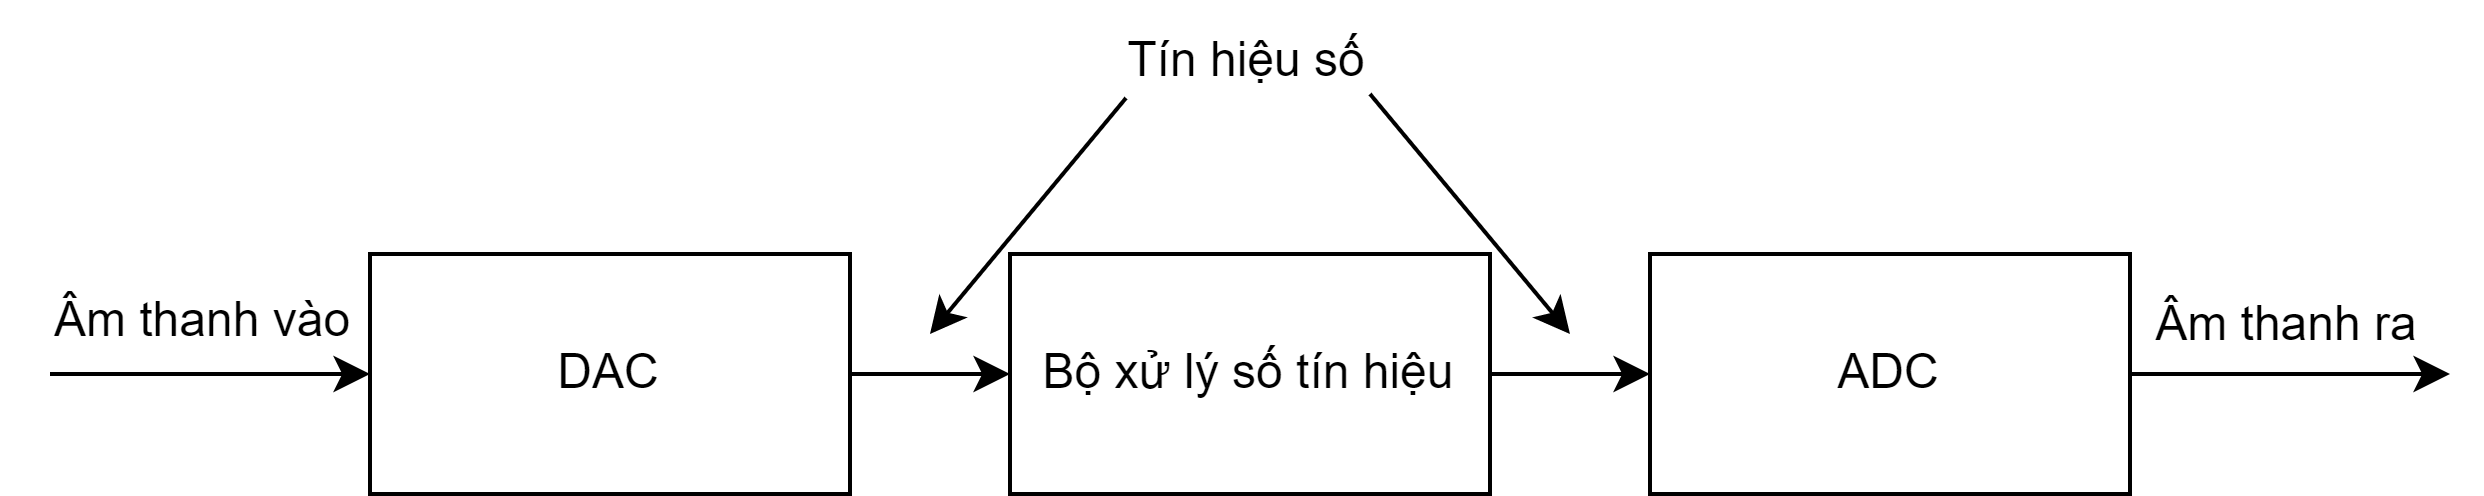
\includegraphics[width=15cm]{Images/top.png}
    \caption[Sơ đồ khối của hệ thống]{\bfseries \fontsize{12pt}{0pt}\selectfont Sơ đồ tổng quan hệ thống xử lí âm thanh số}
    \label{hinh21}
\end{figure}

Quá trình số hóa gồm 3 bước theo thứ tự sau: lấy mẫu, lượng tử và mã hóa. Trong đó, lấy mẫu là lấy các giá trị của tín hiệu tại các thời điểm rời rạc. Do đó, lấy mẫu còn gọi là rời rạc hóa. Tiếp theo, lượng tử hóa là làm gần đúng giá trị của tín hiệu tại thời điểm lấy mẫu với các mức lượng tử (giá trị rời rạc). Lượng tử hóa được xác định bởi độ chính xác của máy tính. Cuối cùng, mã hóa là biểu diễn một số theo hệ thống nhị phân mà máy tính có thể đọc được\cite{xulytinhieusobook}. Ba quá trình trên sẽ được tích hợp và thực hiện trên bộ ADC.

Bộ chuyển đổi tương tự số có 3 kiến trúc phổ biến hiện tại đang được sử dụng là 
Sigma Delta ADC, Successive Approximation ADC (SAR ADC) và Pipelined ADC.
Mỗi kiến trúc có các đặc điểm khác nhau – một số tốt hơn trong việc hỗ trợ độ chính xác của độ phân giải cao, trong khi những kiến trúc khác hỗ trợ tốt hơn cho tốc độ lấy mẫu cao (bảng \ref{bang21}). Cho nên mỗi kiến trúc sẽ được sử dụng trong các ứng dụng khác nhau.
\begin{table}[h!]
\centering
\caption[So sánh giữa các kiến trúc ADC]{\bfseries\fontsize{12pt}{0pt}\selectfont So sánh giữa các kiến trúc ADC}
\begin{tabular}{|c|c|c|c|}
\hline 
\bfseries  Kiến trúc   &\bfseries Tốc độ lấy mẫu   &\bfseries Độ phân giải \hspace{0pt}   & \bfseries Khác\hspace{0pt}\\
\hline 
\multicolumn{1}{|l|}{\begin{tabular}[c]{@{}l@{}}\textbf{SAR}\\ ADS7xxx\\ ADS8xxx\end{tabular}} & \multicolumn{1}{l|}{\begin{tabular}[c]{@{}l@{}}$\leq 4 Msps$\\ $\leq 1.25 Msps$\end{tabular}} & \multicolumn{1}{l|}{\begin{tabular}[c]{@{}l@{}}$\leq 16 bit$\\ $\leq 18 bit$\end{tabular}} & \multicolumn{1}{l|}{\begin{tabular}[c]{@{}l@{}}Dễ dàng sử dụng\\ Độ trễ bằng 0\\ Công suất thấp\end{tabular}} \\ \hline
\multicolumn{1}{|l|}{\begin{tabular}[c]{@{}l@{}}\textbf{Delta-Sigma}\\ ADS10xx/11xx\\ ADS12xx\\ ADS13xx\\ ADS16xx\end{tabular}} & \multicolumn{1}{l|}{\begin{tabular}[c]{@{}l@{}}$\leq 4 Ksps$\\ $\leq 4 Msps$\\ $\leq 10 Msps$\end{tabular}} & \multicolumn{1}{l|}{\begin{tabular}[c]{@{}l@{}}$> 24 bit$\\ $\leq 24 bit$\\ $\leq 16 bit$\end{tabular}} & \multicolumn{1}{l|}{\begin{tabular}[c]{@{}l@{}}Độ phân giải cao\\ Tính tích hợp cao\end{tabular}} \\ \hline
\multicolumn{1}{|l|}{\textbf{Pipeline}} & \multicolumn{1}{l|}{\begin{tabular}[c]{@{}l@{}}$\leq 200 Msps$\\ $\leq 250 Msps$\\ $\leq 1000 Msps$\end{tabular}} & \multicolumn{1}{l|}{\begin{tabular}[c]{@{}l@{}}$\leq 16 bit$\\ $\leq 14 bit$\\ $\leq 12 bit$\end{tabular}} & \multicolumn{1}{l|}{\begin{tabular}[c]{@{}l@{}}Tốc độ cao\\ Công suất cao\end{tabular}} \\ \hline
\end{tabular} 
\label{bang21}
\end{table}

Vì dải âm thanh nghe trong ngưỡng nghe có tần số không cao (20 – 20000 Hz) nằm trong khả năng lấy mẫu của bộ điều chế Delta Sigma và trong các ứng dụng âm thanh được mã hóa trong khoảng từ 16 – 24 bit. Do đó, kiến trúc Delta Sigmal sẽ phù hợp cho việc số hóa âm thanh hơn các kiến trúc còn lại.

Một thiết bị điển hình sử dụng kiến trúc Sigma Delta (SD) là MEMS Microphone, 
(MicroelectromechanicalSystem Microphone) thiết bị này có thể được tìm thấy phổ biến trên các điện thoại di động, các máy ghi âm hoặc các thiết bị thu thanh không sử yêu cầu về chất lượng âm thanh quá cao nhưng giá thành rẻ và phù hợp với yêu cầu sử dụng. Tín hiệu thu được trên MEMS Microphone có dạng tín hiệu Pulse Density Modulation (PDM), là dạng 1 bit và truyền với tần số cao, giao thức truyền tương ứng có tên là PDM Interface. Một số MEMS Microphone sử dụng giao thức truyền âm thanh là I2S nhưng chỉ là số ít, phần lớn sử dụng PDM.
\begin{figure}[!ht]
    \centering
    \includesvg[width=13cm]{Images/Chuong2/sinewave_to_pdm.svg}
    \caption[Tín hiệu PDM sau khi điều chế sóng sin qua bộ Sigma-Delta]{\bfseries \fontsize{12pt}{0pt}\selectfont Tín hiệu PDM sau khi điều chế sóng sin qua bộ Sigmal-Delta}
    \label{hinh22}
\end{figure}

Hình \ref{hinh22} cho ta thấy được tín hiệu sóng Sin (màu đỏ) được điều chế qua bộ Sigma-Delta bậc nhất với tỷ lệ lấy mẫu là 16 thu được tín hiệu PDM (màu xanh).
\subsubsection{Điều chế mật độ xung - PDM là gì?}

Điều chế mật độ xung (Pulse Density Modulation) là một phương pháp biểu diễn tín hiệu số bằng cách thay đổi mật độ xung (pulse density) của tín hiệu xung điện. PDM được sử dụng để mô tả các tín hiệu âm thanh và được sử dụng trong các ứng dụng âm thanh số, chẳng hạn như hệ thống âm thanh trên ô tô, thiết bị di động, hệ thống truyền thông v.v.

Trong PDM, tín hiệu âm thanh được biểu diễn bằng một chuỗi các xung điện, mỗi xung có độ rộng như nhau nhưng với mật độ xung khác nhau tại các thời điểm khác nhau (hình \ref{hinh22}). Trong đó, mật độ xung được thể hiện bằng số lượng xung được phát ra trong một khoảng thời gian cố định. Có thể thu được tín hiệu PDM từ bộ chuyển đổi tương tự số Sigma-Delta, quá trình này sẽ được trình bày ở các phần sau.

\subsubsection{Bộ chuyển đổi tương tự số Sigma-Delta}
Bộ chuyển đổi Sigma-Delta ($\Sigma\Delta$ Converter) cơ bản là một hệ thống lấy mẫu 1 bit. Tín hiệu tương tự đầu vào cần phải tương đối chậm để bộ chuyển đổi có thể lấy mẫu tín hiệu đó nhiều lần. Một kỹ thuật được gọi là lấy mẫu quá mức (oversampling) - tốc độ lấy mẫu (sample rate) nhanh hơn hàng trăm lần so với kết quả số được thu ở đầu ra. Mỗi mẫu được tích lũy theo thời gian và được lấy trung bình với các tín hiệu đầu vào khác thông qua bộ lọc số (digital filter) và bộ lọc giảm mẫu số (decimation filter).\cite{8227915}

Các thành phần chính của bộ chuyển đổi Sigma-Delta bao gồm bộ điều chế Sigma-Delta, bộ lọc kỹ thuật số và bộ lọc decimation. Trong đó, decimation filters là các bộ lọc số được sử dụng để giảm mẫu số của tín hiệu số cũng như giảm tần số lấy mẫu của tín hiệu. Decimation là quá trình giảm mẫu số của tín hiệu số, điều này thường được thực hiện để giảm tải cho bộ xử lý hoặc để giảm băng thông tín hiệu. 
\begin{figure}[!ht]
    \centering
    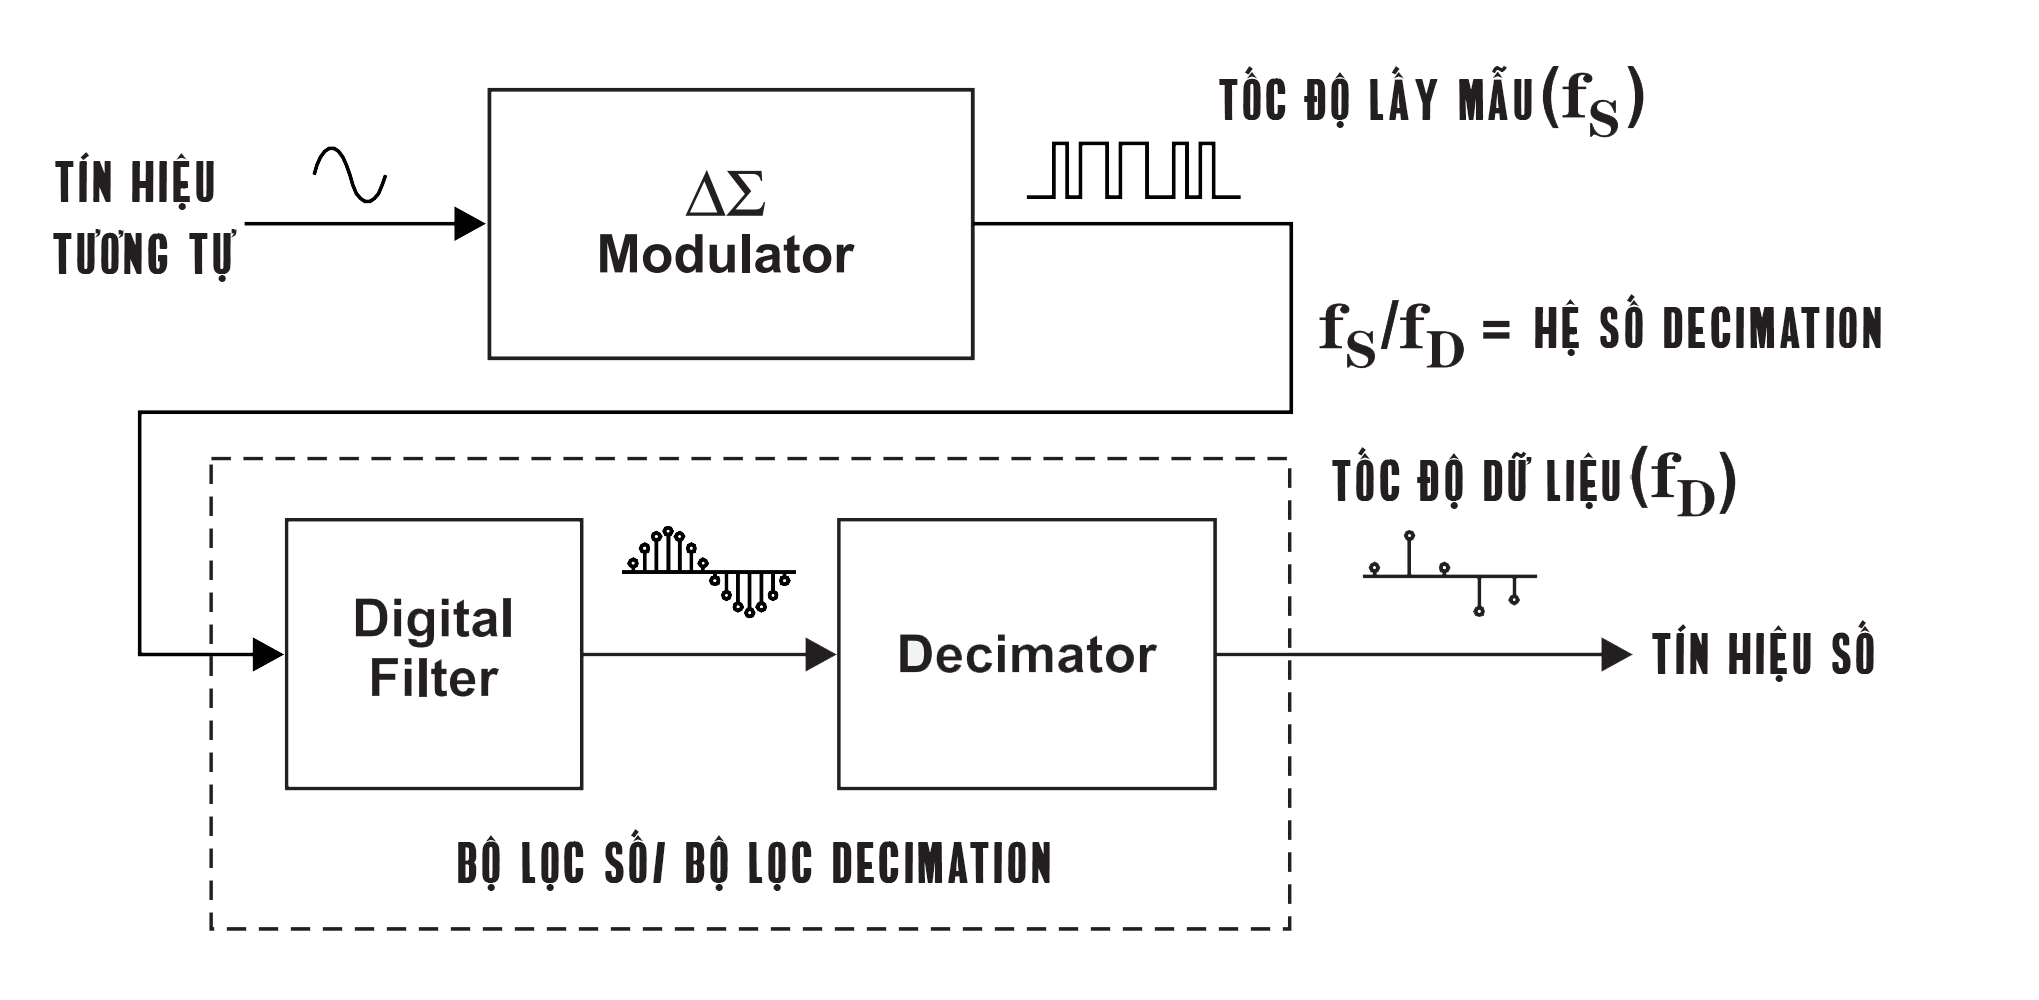
\includegraphics[width=12cm]{Images/Chuong2/DAC-SD.png}
    \caption[Cấu trúc của bộ ADC sử dụng Sigma-Delta]{\bfseries \fontsize{12pt}{0pt}\selectfont Cấu trúc của bộ ADC sử dụng Sigma-Delta}
    \label{hinh23}
\end{figure}

Bộ điều chế Sigma-Delta được thể hiện trong hình \ref{hinh23}, nó lấy thô tín hiệu đầu vào ở tốc độ rất cao thành luồng 1 bit. Sau đó, bộ lọc kỹ thuật số và bộ lọc decimation lấy dữ liệu lấy mẫu này và chuyển đổi thành tín hiệu số có tần số thấp hơn và đồng thời có độ phân giải cao. Trong một bộ chuyển đổi thì sẽ tốc độ lấy mẫu $f_S$ (sample rate) và tốc độ đầu ra dữ liệu $f_D$ (data rate).

\subsubsection{Điều chế Sigma-Delta}
Bộ điều chế Sigma-Delta là "trái tim" của bộ Sigma-Delta ADC. Nó có thể đáp ứng để số hóa tín hiệu đầu vào tương tự và giảm nhiễu ở tần số thấp hơn. Trong giai đoạn này, kiến trúc thực hiện một chức năng gọi là định hình nhiễu (noise shaping) để đẩy nhiễu tần số thấp lên các tần số cao hơn ở những nơi nó nằm ngoài dải tần quan tâm. Định dạng nhiễu là một trong những lý do khiến bộ chuyển đổi Sigma-Delta rất phù hợp cho các phép đo tần số thấp, độ chính xác cao. \cite{Baker2011HowDA}
\begin{figure}[!ht]
    \centering
    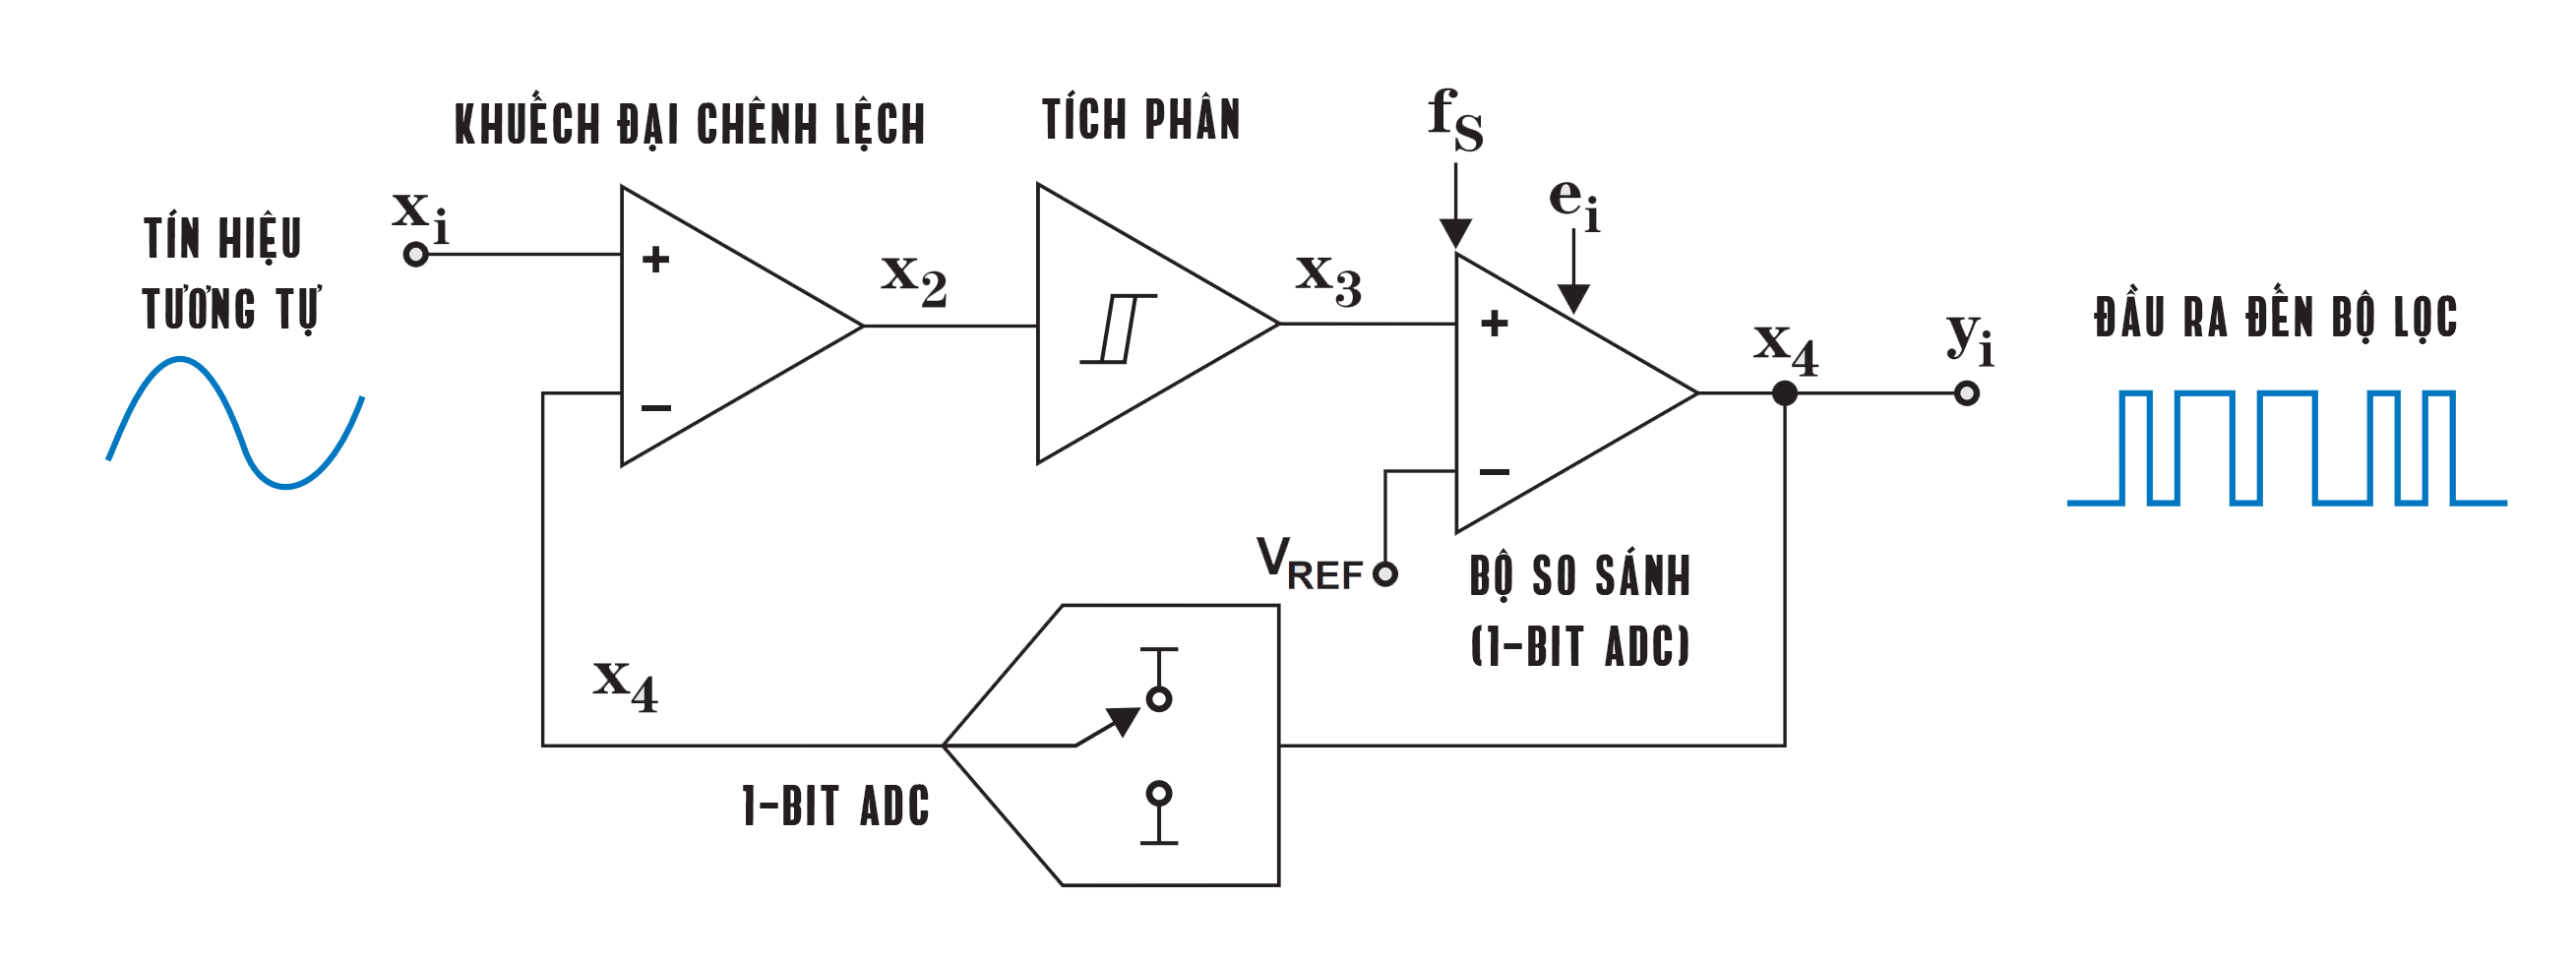
\includegraphics[width=13cm]{Images/Chuong2/kientruc_1st.png}
    \caption[Kiến trúc của Sigma-Delta bậc nhất trong miền thời gian]{\bfseries \fontsize{12pt}{0pt}\selectfont Kiến trúc của Sigma-Delta bậc nhất trong miền thời gian}
    \label{hinh24}
\end{figure}

Có hai cách để xem bộ điều biến Sigma-Delta là trong miền thời gian hoặc trong miền tần số. Sơ đồ khối miền thời gian trong hình \ref{hinh24} cho thấy cơ chế của bộ điều chế Sigma-Delta bậc nhất. Các bộ điều chế chuyển đổi tín hiệu đầu vào tương tự thành sóng xung được điều chế, một bit và ở tốc độ cao. Quan trọng hơn, phân tích tần số trong hình \ref{hinh25} cho thấy cách bộ điều biến ảnh hưởng đến nhiễu trong hệ thống và tạo điều kiện tạo ra kết quả có độ phân giải cao hơn.
\begin{figure}
    \centering
    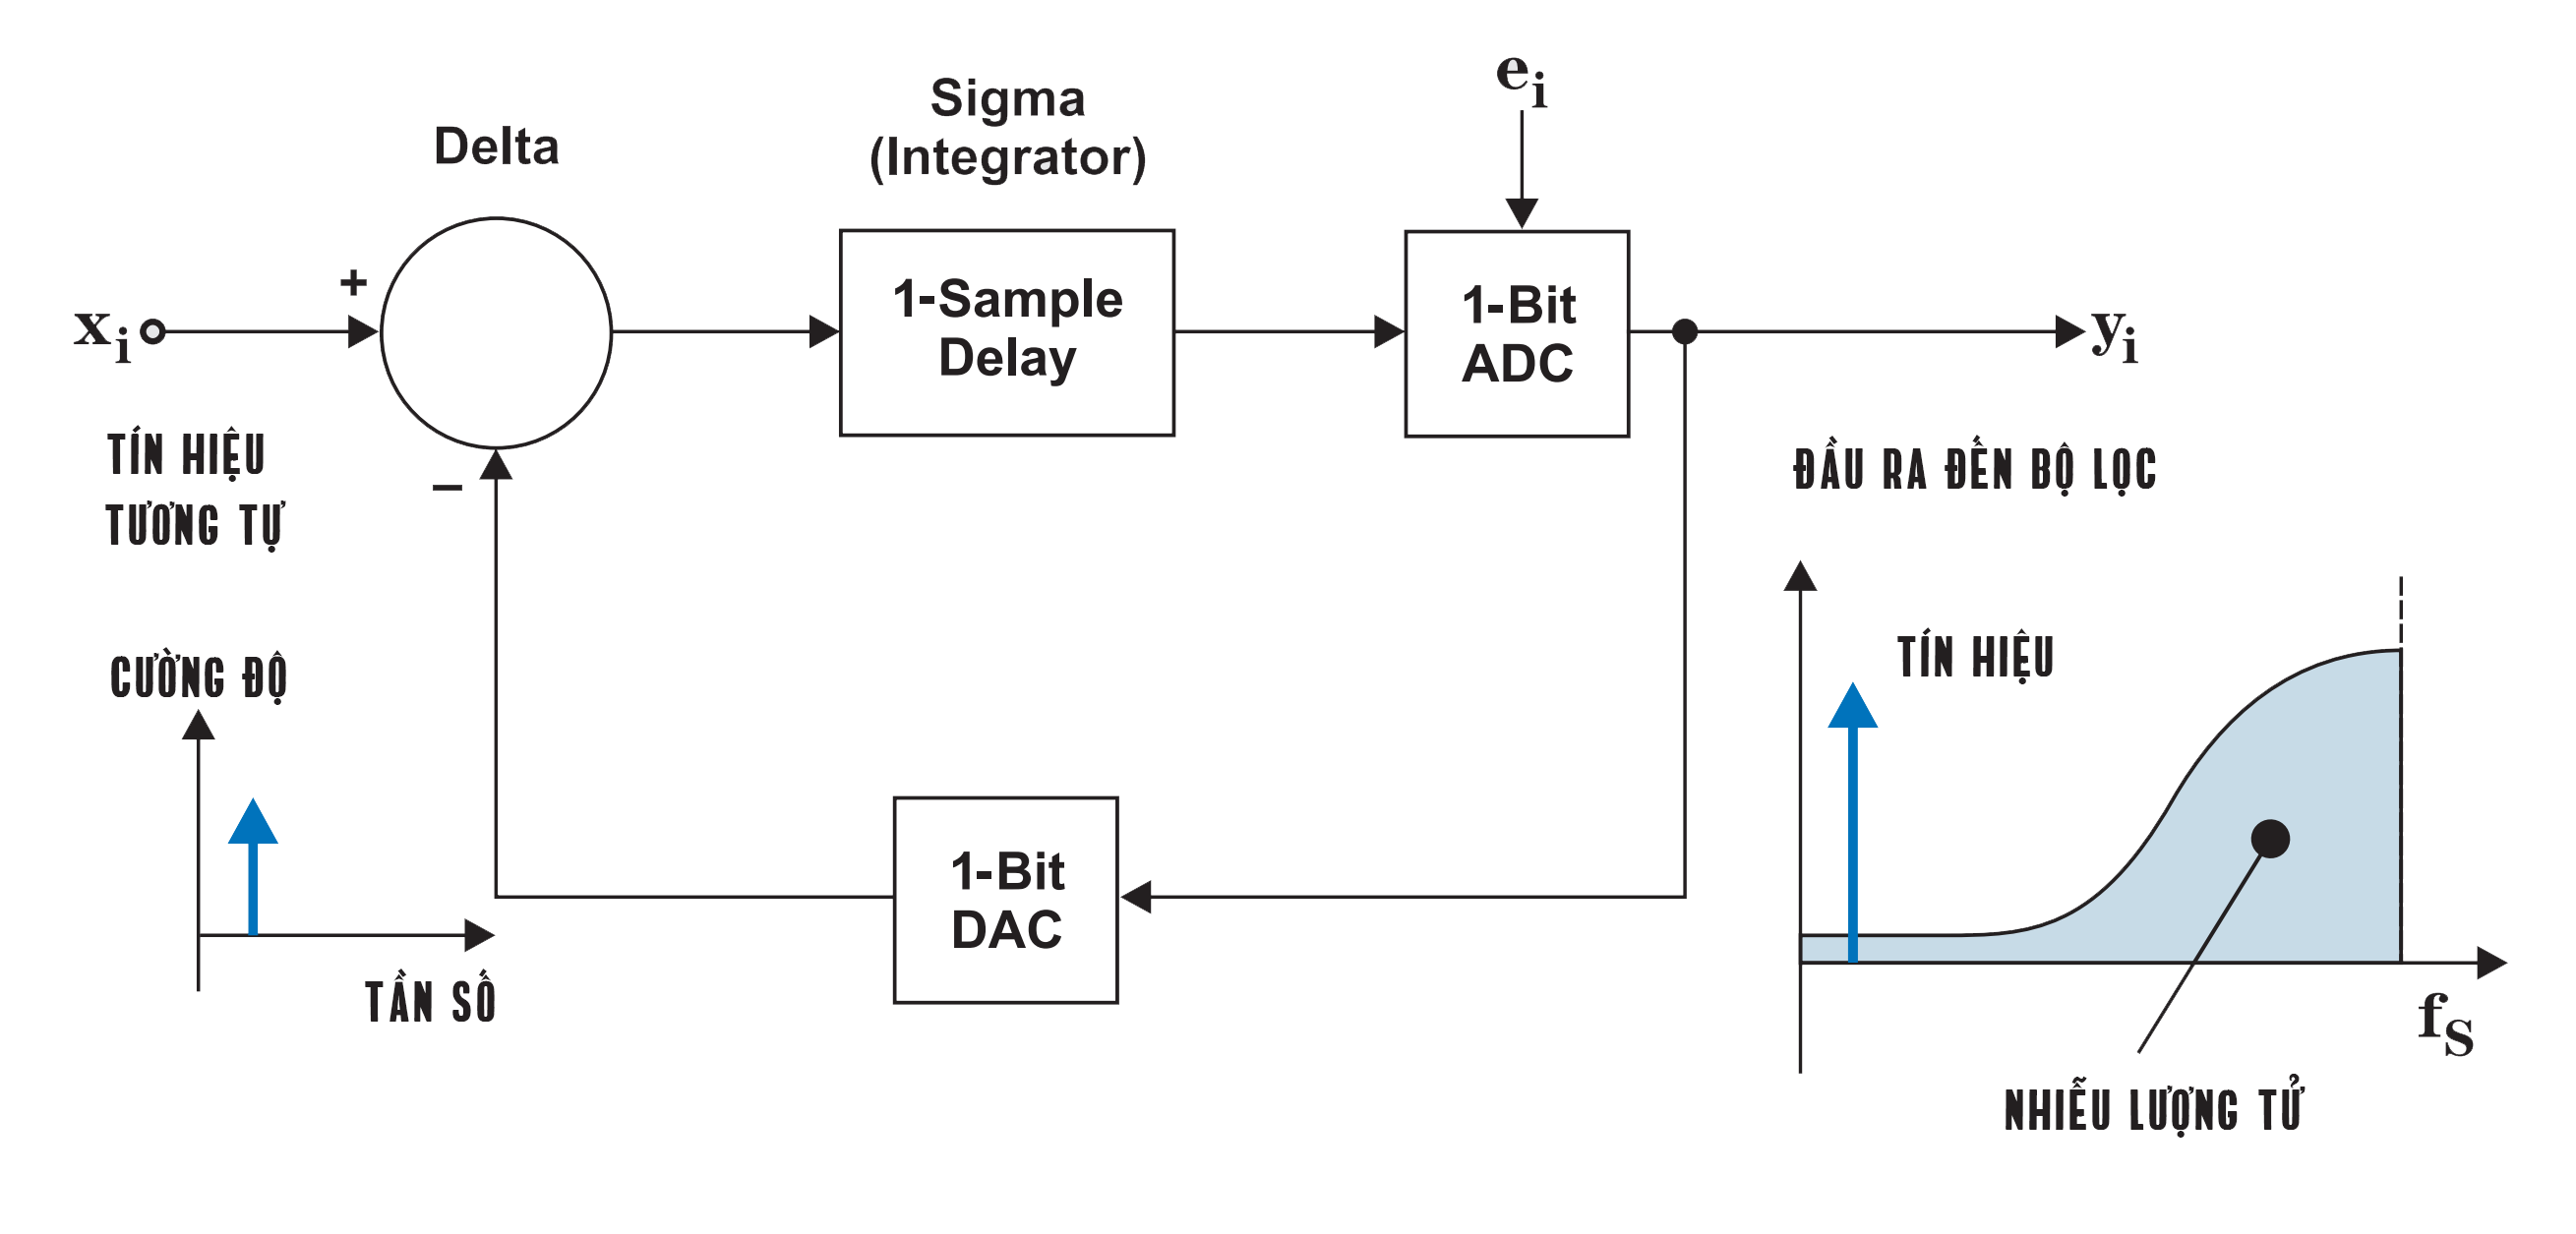
\includegraphics[width=13cm]{Images/Chuong2/kientruc_1st_pho.png}
    \caption[Kiến trúc của Sigma-Delta bậc nhất trong miền tần số]{\bfseries \fontsize{12pt}{0pt}\selectfont Kiến trúc của Sigma-Delta bậc nhất trong miền tần số}
    \label{hinh25}
\end{figure}

Bộ điều biến Sigma-Delta thể hiện trong hình \ref{hinh24} thu được nhiều mẫu tín hiệu đầu vào để tạo ra luồng mã 1 bit. Đồng hồ hệ thống thực hiện tốc độ lấy mẫu với tần số $f_S$, kết hợp với bộ so sánh 1 bit của bộ điều chế.

Theo cách này, hoạt động lượng tử hóa của bộ điều biến Sigma-Delta được tạo ra ở tốc độ lấy mẫu cao bằng với tốc độ của đồng hồ hệ thống. Giống như tất cả các bộ lượng tử hóa, bộ điều chế Sigma-Delta tạo ra một luồng các giá trị kỹ thuật số biểu thị điện áp 
của đầu vào, trong trường hợp này là luồng 1 bit. Do đó, tỷ lệ giữa số 1 và 0 biểu thị điện áp tương tự đầu vào. Không giống như hầu hết các bộ lượng tử hóa, bộ điều chế Sigmal-Delta bao gồm một bộ tích phân, có tác dụng định hình nhiễu lượng tử hóa thành các tần số cao hơn. Do đó, phổ của nhiễu ở đầu ra của bộ điều biến không bằng phẳng.

Trong miền thời gian, điện áp đầu vào tương tự và đầu ra của bộ khuếch đại là khác nhau. Điện áp tại $x_2$ được đưa vào bộ tích phân, đầu ra tiến triển theo hướng âm hoặc dương. Độ dốc và hướng của tín hiệu tại $x_3$ phụ thuộc vào dấu và độ lớn của điện áp tại $x_2$. Tại thời điểm điện áp tại $x_3$ bằng với điện áp tham chiếu của bộ so sánh, đầu ra của bộ so sánh chuyển từ âm sang dương hoặc dương sang âm, tùy thuộc vào trạng thái ban đầu của nó. Giá trị đầu ra của bộ so sánh, $x_4$, được đặt xung nhịp trở lại vào DAC 1 bit, cũng như đưa đầu ra $y_i$ cho bộ lọc số. Tại thời điểm đầu ra của bộ so sánh chuyển từ cao xuống thấp hoặc ngược lại, DAC 1 bit sẽ phản hồi bằng cách thay đổi điện áp đầu ra tương tự của bộ khuếch đại chênh lệch. Điều này tạo ra một điện áp đầu ra khác ở $x_2$, làm cho bộ tích phân tiến triển theo hướng ngược lại. Tín hiệu đầu ra miền thời gian này là biểu diễn sóng xung của tín hiệu đầu vào ở tốc độ lấy mẫu ($f_S$).

\begin{equation}\label{pt21}
    y_i = x_{i - 1} + (e_i - e_{i - 1})
\end{equation}

 Trong miền thời gian, ADC 1 bit số hóa tín hiệu thành mã đầu ra thô, 1 bit tạo ra nhiễu lượng tử hóa của bộ chuyển đổi. Đầu ra của bộ điều chế bằng đầu vào cộng với nhiễu lượng tử hóa, $e_i - e_{i-1}$. Với $y_i$ được biểu diễn như phương trình \ref{pt21}. Như công thức này cho thấy, nhiễu lượng tử hóa là sự khác biệt giữa lỗi lượng tử hóa hiện tại ($e_i$) và lỗi lượng tử hóa trước đó ($e_{i - 1}$). Hình \ref{hinh25} minh họa vị trí tần số của nhiễu lượng tử hóa này.

Trong miền tần số, các xung đầu ra miền thời gian xuất hiện dưới dạng tín hiệu đầu vào và nhiễu định hình. Các đặc điểm nhiễu trong hình \ref{hinh25} là chìa khóa để hiểu hoạt động tần số của bộ điều chế và khả năng của DS ADC để đạt được độ phân giải cao. Nhiễu trong bộ điều chế được chuyển ra tần số cao hơn. Hình \ref{hinh25} cho thấy nhiễu lượng tử hóa đối với bộ điều chế bậc nhất bắt đầu thấp ở $0 Hz$, tăng nhanh và sau đó giảm xuống ở giá trị tối đa tại tần số lấy mẫu của bộ điều chế ($f_S$).

\begin{figure}[!ht]
    \centering
    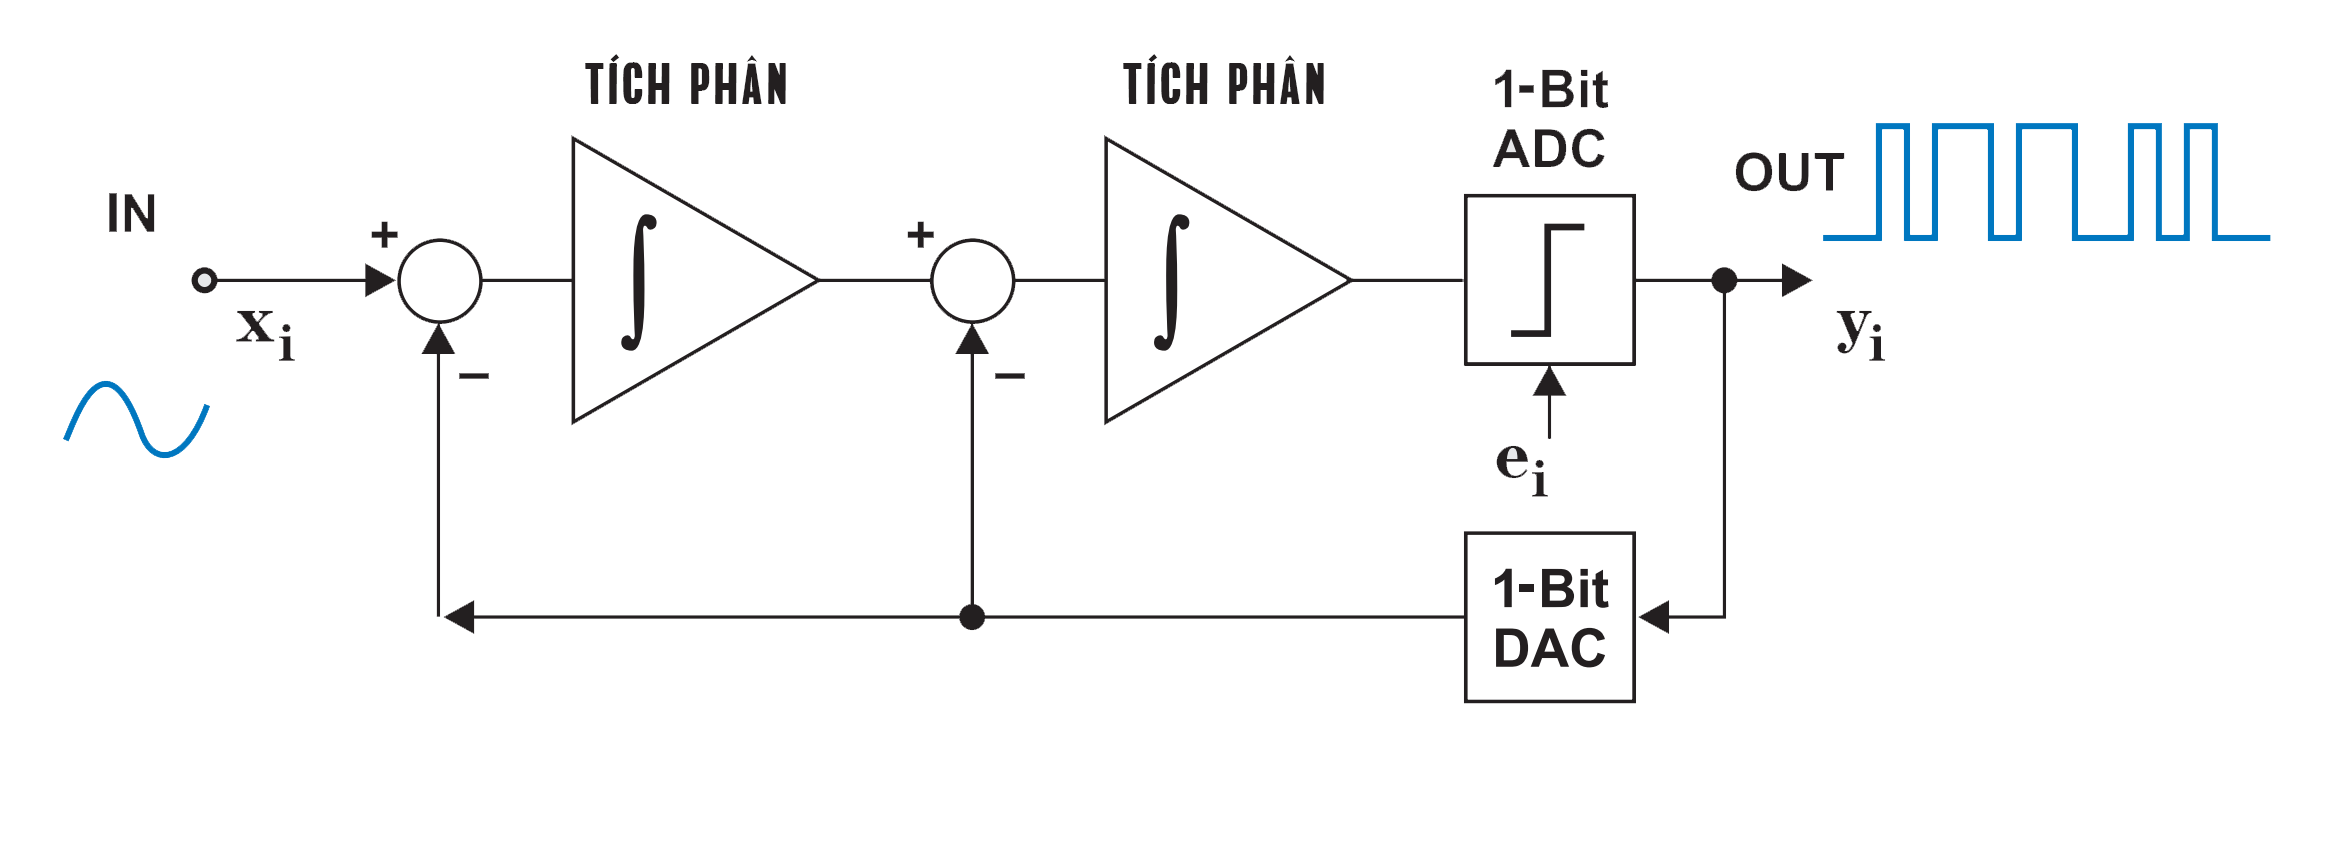
\includegraphics[width=13cm]{Images/Chuong2/kientruc_2st.png}
    \caption[Kiến trúc của bộ điều chế Sigma-Delta bậc hai]{\bfseries \fontsize{12pt}{0pt}\selectfont Kiến trúc của bộ điều chế Sigma-Delta bậc hai}
    \label{hinh26}
\end{figure}

Sử dụng mạch tích phân hai lần thay vì chỉ một lần là một cách tuyệt vời để giảm nhiễu lượng tử hóa trong dải của bộ điều chế. Hình \ref{hinh26} cho thấy bộ điều chế bậc hai, 1 bit có hai bộ tích phân thay vì một. Với ví dụ về bộ điều biến bậc hai này, thuật ngữ nhiễu không chỉ phụ thuộc vào lỗi trước đó mà cả hai lỗi trước đó.

Một số nhược điểm của thứ hai hoặc đa thứ tự bộ điều biến bao gồm tăng độ phức tạp, nhiều vòng lặp, và tăng độ khó thiết kế. Tuy nhiên, hầu hết các bộ điều chế Sigma-Delta đều có bậc cao hơn, với ứng dụng âm thanh thì bộ điều chế thường sẽ bậc hai đến bậc sáu.

\begin{figure}[!ht]
    \centering
    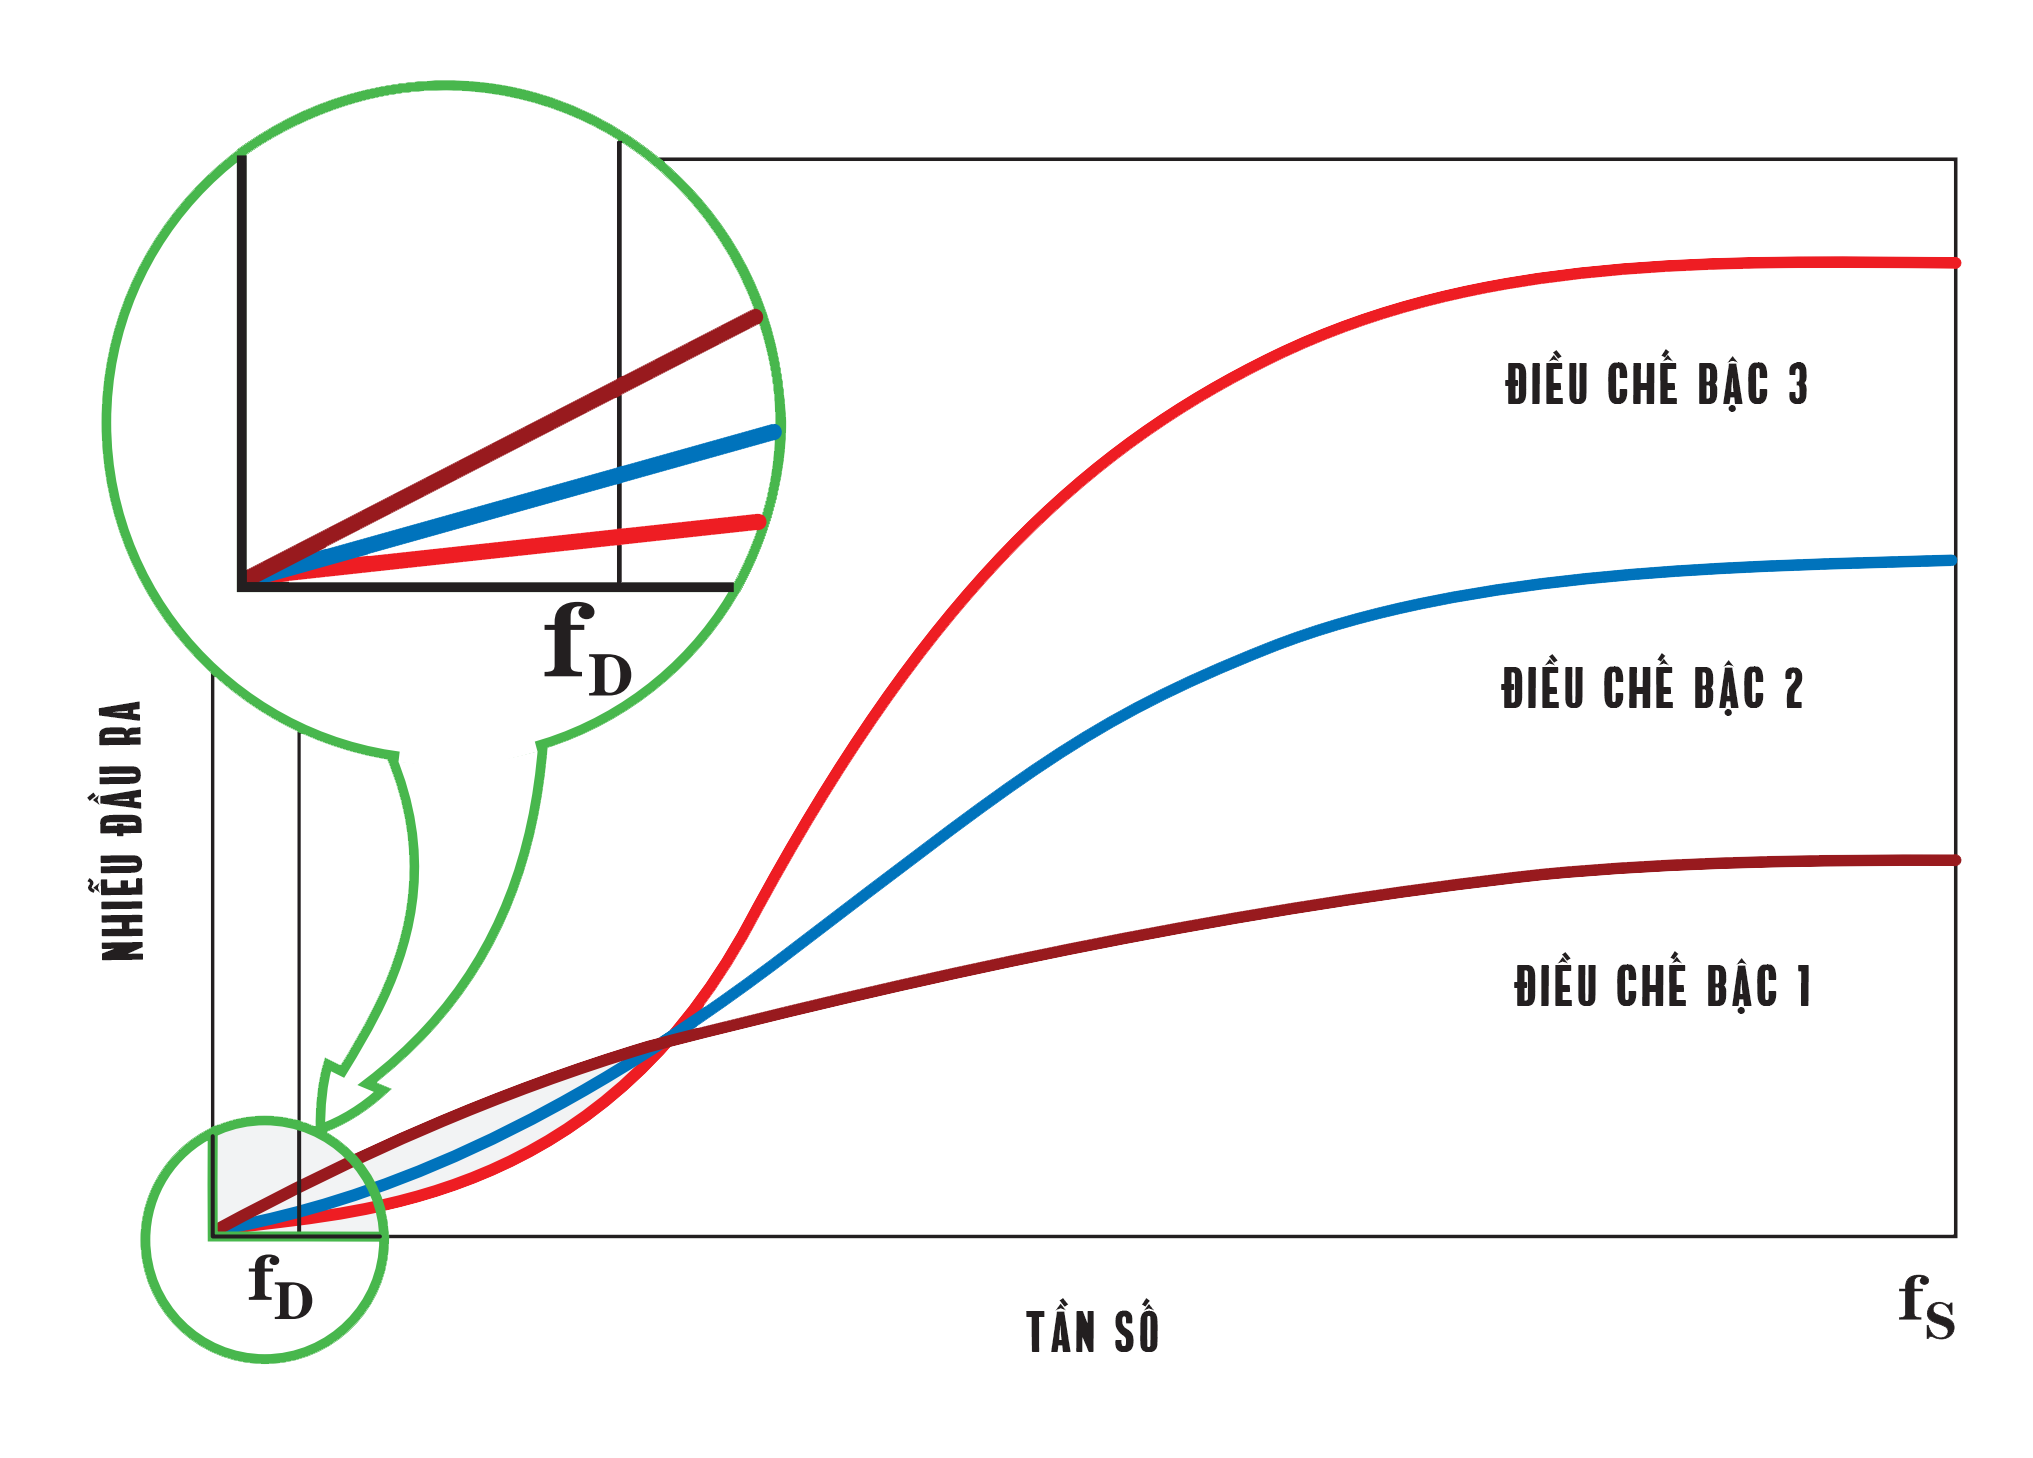
\includegraphics[width=12cm]{Images/Chuong2/bieudoDS.png}
    \caption[Biểu đồ thể hiện nhiễu ở đầu ra ở các kiến trúc Sigma-Delta khác nhau]{\bfseries \fontsize{12pt}{0pt}\selectfont Biểu đồ thể hiện nhiễu ở đầu ra ở các kiến trúc Sigma-Delta khác nhau}
    \label{hinh27}
\end{figure}

Các bộ điều chế đa bậc định hình nhiễu lượng tử ở các tần số thậm chí còn cao hơn so với các bộ điều biến bậc thấp. Trong hình \ref{hinh27}, đường cao nhất ở tần số $f_S$ thể hiện đáp ứng nhiễu của bộ điều chế bậc ba. Lưu ý rằng đầu ra của bộ điều chế này có nhiễu rất lớn ở tần số lấy mẫu của nó là $f_S$. Tuy nhiên, ở các tần số thấp hơn, dưới $f_D$ và gần mức tín hiệu đầu vào, bộ điều chế bậc ba có nhiễu thấp. $f_D$ là tần số chuyển đổi của bộ lọc số/ bộ lọc decimation.
\subsubsection{Điều chế Sigma-Delta cho tín hiệu âm thanh}
Âm thanh trong ngưỡng nghe được của con người nằm trong khoảng $20Hz$ đến 
$20kHz$, nếu thực hiện lấy mẫu âm thanh trong ngưỡng nghe ta cần sử dụng tần số lấy 
mẫu ít nhất bằng 2 lần tần số âm thanh lớn nhất. Đó là lý do tại sao hầu hết âm thanh được ghi ở tốc độ mẫu $44,1kHz$ hoặc $48kHz$.

Số bit trên mẫu (độ phân giải) là 1 thông số ảnh hưởng đến độ sai khác của giá trị số thu được so với ngưỡng thực tế của tín hiệu tương tự. Số bit càng lớn thì sự sai khác so với tín hiệu tương tự càng nhỏ.

\begin{figure}[!ht]
    \centering
    \includesvg[width=13cm]{Images/Chuong2/quantization_noise_8.svg}
    \caption[Sóng sin được lượng tử hóa với 8 mức]{\bfseries \fontsize{12pt}{0pt}\selectfont Sóng sin được lượng tử hóa với 8 mức}
    \label{h_quantization_noise_8}
\end{figure}
Trong biểu đồ hình \ref{h_quantization_noise_8}, sóng hình sin được lượng tử hóa thành 8 mức riêng biệt (3 bit). Cách rõ ràng để giảm tiếng ồn lượng tử hóa là tăng số lượng bit. Ở mức 256 (8 bit), hầu như không nhìn thấy nhiễu trên biểu đồ tuyến tính (hình \ref{h_quantization_noise_256}).

\begin{figure}[!ht]
    \centering
    \includesvg[width=13cm]{Images/Chuong2/quantization_noise_256.svg}
    \caption[Sóng sin được lượng tử hóa với 256 mức]{\bfseries \fontsize{12pt}{0pt}\selectfont Sóng sin được lượng tử hóa với 256 mức}
    \label{h_quantization_noise_256}
\end{figure}

Âm thanh cấp độ CD sử dụng âm thanh 16 bit. Âm thanh chuyên nghiệp thường sử dụng 24 bit. Tuy nhiên, có thể đánh đổi số bit lấy tốc độ xung nhịp.

Với tín hiệu PDM như đã trình bày ở trên, dạng tín hiệu đầu ra là 1 bit biểu thị 2 giá trị, khi dùng 1 bit để lấy mẫu tín hiệu âm thanh thì phần nhiễu lượng tử là rất lớn, tín hiệu PDM là một trong số đó.

Hình \ref{hinh22} là một ví dụ về sóng hình sin PCM 16kHz với tốc độ lấy mẫu 48kHz được chuyển đổi thành PDM bằng bộ chuyển đổi Sigma-Delta bậc một và tỷ lệ oversampling 16.

Chỉ tăng tốc độ lấy mẫu quá mức (oversampling) và giảm số lượng bit đầu ra trong bộ chuyển đổi A/D không tự động giảm nhiễu lượng tử hóa. Trong thực tế, tiếng ồn là không thể tránh khỏi. Tuy nhiên, có thể đẩy nhiễu này vào các thành phần tần số nằm ngoài dải tần của tín hiệu đầu vào ban đầu, sau đó dùng bộ lọc thông thấp sẽ dễ dàng khôi phục được tín hiệu ban đầu.
\begin{figure}[!ht]
    \centering
    \includesvg[width=13cm]{Images/Chuong2/sinewave_pdm_psd.svg}
    \caption[Mật độ phổ công suất của tín hiệu PDM]{\bfseries \fontsize{12pt}{0pt}\selectfont Mật độ phổ công suất của tín hiệu PDM}
    \label{sinewave_pdm_psd}
\end{figure}

Hình \ref{sinewave_pdm_psd} mô tả mật độ phổ công suất của tín hiệu PDM ở trên (hình \ref{hinh22}). Chúng ta có thể thấy rõ, tín hiệu đã lấy mẫu nằm ở bên trái đường xanh lục ở vị trí $24kHz$ ($1/2$ của $48kHz$ - tốc độ lấy mẫu ban đầu). Đó là nơi có tăng đột biến - sóng sin ban đầu, còn lại là nhiễu.

Để giải quyết vấn đề nhiễu lượng tử, bộ điều chế Sigma-Delta sẽ giải quyết bằng cách sử dụng kiến trúc có bậc cao hơn và tăng tăng tần số lấy mẫu lên gấp nhiều lần so với tần số lớn nhất trong dải tín hiệu cần được lấy mẫu - Oversampling rate. Các cách trên sẽ trình bày ở mục \ref{inc_order} và \ref{inc_sam}.
\paragraph{Sử dụng bộ điều chế Sigma-Delta có số bậc cao} \label{inc_order}
\begin{figure}
    \centering
    \includesvg[width=14cm]{Images/Chuong2/sinewave_to_pdm_different_orders.svg}
    \caption[Tín hiệu PDM tạo ra từ sóng sin với số bậc của bộ điều chế tăng dần]{\bfseries \fontsize{12pt}{0pt}\selectfont Tín hiệu PDM tạo ra từ sóng sin với số bậc của bộ điều chế tăng dần}
    \label{sinewave_to_pdm_different_orders}
\end{figure}
\begin{figure}
    \centering
    \includesvg[width=14cm]{Images/Chuong2/sinewave_to_pdm_different_osr.svg}
    \caption[Tín hiệu PDM tạo ra từ sóng sin với bộ điều chế bậc 4 và tỷ lệ Oversampling tăng dần]{\bfseries \fontsize{12pt}{0pt}\selectfont Tín hiệu PDM tạo ra từ sóng sin với bộ điều chế bậc 4 và tỷ lệ Oversampling tăng dần}
    \label{sinewave_to_pdm_different_osr}
\end{figure}
\begin{figure}
    \centering
    \includesvg[width=15cm]{Images/Chuong2/sinewave_pdm_psd_different_orders.svg}
    \caption[Mật độ phổ công suất của tín hiệu PDM ở các kiến trúc khác nhau]{\bfseries \fontsize{12pt}{0pt}\selectfont Mật độ phổ công suất của tín hiệu PDM ở các kiến trúc khác nhau}
    \label{sinewave_pdm_psd_different_orders}
\end{figure}
\begin{figure}[ht!]
    \centering
    \includesvg[width=14cm]{Images/Chuong2/sinewave_pdm_psd_different_osr.svg}
    \caption[Mật độ phổ công suất của tín hiệu PDM ở các Oversampling khác nhau]{\bfseries \fontsize{12pt}{0pt}\selectfont Mật độ phổ công suất của tín hiệu PDM ở các Oversampling khác nhau}
    \label{sinewave_pdm_psd_different_osr}
\end{figure}
Như đã trình bày ở trên, việc sử dụng mạch tích phân nhiều lần thay vì chỉ một lần là một cách cực kỳ hiệu quả để giảm nhiễu lượng tử hóa trong dải của bộ điều chế.


Ở hình \ref{sinewave_to_pdm_different_orders}, không sự khác biệt nào để phân biệt tín hiệu khi tăng số bậc của bộ điều chế Sigma-Delta. 

Nhưng ở trường hợp này trong miền tần số sẽ có những thay đổi rõ rệt. Mặc dùng tỷ lệ Oversamling không đổi nhưng $SNR$ vẫn tăng từ $35dB$ lên $50.2dB$ (hình \ref{sinewave_pdm_psd_different_orders}).  Việc tăng số bậc sẽ không tối ưu vì khi ở một bậc nào đó chỉ số $SNR$ sẽ ngừng tăng, đối với trường hợp trên thì $SNR$ tối đa là $51dB$.

Mặc dù bộ chuyển đổi Sigma-Delta bậc cao sẽ có kiến trúc phức tạp hơn và tại một số thời điểm chúng trở nên khó giữ ổn định nhưng chúng đã giải quyết được vấn đề nhiễu lượng tử ở vùng cần lấy thông tin. Hầu hết các micrô PDM hiện đại đều sử dụng bộ chuyển đổi Sigma-Delta bậc 4.


\paragraph{Tăng tỷ lệ oversampling} \label{inc_sam}
Tác động của oversampling sẽ làm tăng tỉ số $SNR$ trong dải tần tín hiệu cần thu.

Việc tăng tỷ lệ oversampling từ 16 lên 64, lần này tín hiệu PDM thay đổi rõ rệt ở miền thời gian (hình \ref{sinewave_to_pdm_different_osr}), mật độ tín hiệu đầu ra cũng sẽ dày hơn so với ban đầu.

Hệ số $SNR$ tăng lên đáng kể, từ $50.2dB$ ở 16x lên $102.8dB$ ở 64x (hình \ref{sinewave_pdm_psd_different_osr}).

Từ mục \ref{inc_order} và \ref{inc_sam}, việc sử dụng bộ điều chế Sigma-Delta bậc 4 và tỷ lệ oversampling 64 là tối ưu nhất cho việc chuyển đổi âm thanh tương tự sang số. Và chính xác đó là kiến trúc mà micro PDM ngày này dùng phổ biến.

\subsection{Xử lí tín hiệu trên nhiều miền tần số}\label{xulynhieumientanso}
Trong một hệ thống xử lý tín hiệu hay điều khiển số, có thể có
một số thiết bị có vận tốc xử lý khác nhau. Như vậy, để có thể kết nối
các thiết bị, cần có phương pháp thay đổi vận tốc xử lý nhằm đồng
bộ hóa hệ thống. Vì ở trong phạm vi của đề tài nên ở trong bài báo cáo chỉ đề cập đến kỹ thuật hạ tốc (Down-Sampling).
\subsubsection{Giới thiệu về định lý Nyquist–Shannon}
Định lý lấy mẫu Nyquist-Shannon là một định lý được sử dụng trong lĩnh vực lý thuyết thông tin, đặc biệt là trong viễn thông và xử lý tín hiệu.
\begin{theorem}\label{dlnq} % Định lý
 Lấy mẫu Nyquist–Shannon: Một hàm số tín hiệu $x(t_n)$ không chứa bất kỳ thành phần tần số nào lớn hơn hoặc bằng một giá trị $f_m$ có thể biểu diễn chính xác bằng tập các giá trị của nó với chu kỳ lấy mẫu $T=1/(2f_m)$.
\end{theorem}

Từ định lý \ref{dlnq}, tần số lấy mẫu phải thoả mãn điều kiện $f_s \geq 2f_m$. Tần số giới hạn $f_s/2$ này được gọi là tần số Nyquist và khoảng $(-f_s/2; f_s/2)$ gọi là khoảng Nyquist. Thực tế, tín hiệu trước khi lấy mẫu sẽ bị giới hạn bằng một bộ lọc để tần số tín hiệu nằm trong khoảng Nyquist.

\subsubsection{Hạ tốc: Giảm mẫu theo hệ số nguyên - Down-Sampling} \label{downsample}
Cho $x_a(t)$ là một tín hiệu tương tự được lấy mẫu với chu kỳ $T$
để cho tín hiệu số $x(n)$. Với điều kiện tần số lấy mẫu đã thỏa điều kiện lấy
mẫu Nyquist thì từ tín hiệu $x(n)$ có thể tái tạo lại tín hiệu $x_a(t)$ chính xác nhất. Để xét trường hợp tổng quát, ta sẽ hạ tốc bởi một số nguyên $M$, tức tăng chu kỳ vận tốc lấy mẫu $T$ thành $T^\prime=MT$, để có tín hiệu số $x_{\downarrow M}(n)$. Nếu vận tốc lấy mẫu $F^\prime_S$ không thỏa điều kiện lấy mẫu Nyquist, rất có thể sẽ có hiện tượng chồng phổ xảy ra, và đây là điều rất cần chú ý. \cite{xulytinhieusobook}\cite{rao2018digital}

\begin{figure}[H]
    \centering
    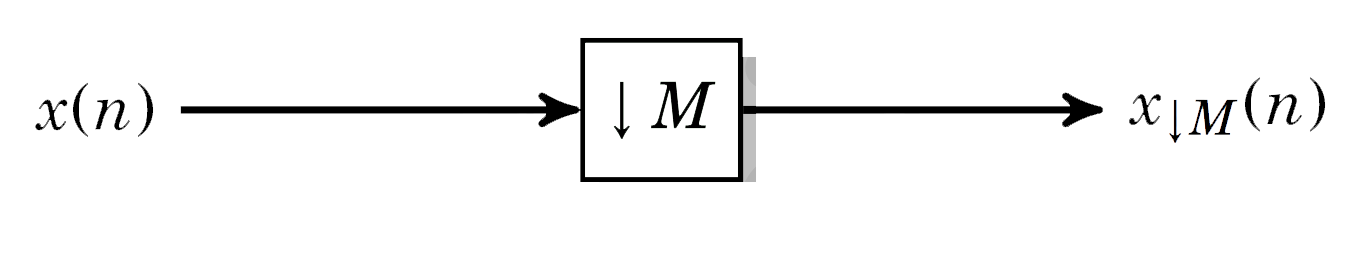
\includegraphics[width=10cm]{Images/Chuong2/downsampling-top.png}
    \caption[Sơ đồ khối của phép hạ tốc]{\bfseries \fontsize{12pt}{0pt}\selectfont Sơ đồ khối của phép hạ tốc}
    \label{downsampling-top}
\end{figure}
Thao tác lấy mẫu được triển khai bằng xác định một trình tự mới cho $x_{\downarrow M}(n)$ trong đó mọi mẫu thứ $M$ của đầu vào được giữ lại và $M-1$ mẫu còn lại sẽ được loại bỏ. Tức là $x_{\downarrow M}(n)$ thu được bằng cách lấy mẫu với chu kỳ $T^\prime$ của $x_a(n)$ được biểu diễn như phương trình \ref{pt22}. Hình \ref{downsampling-top} dùng để mô tả phép toán hạ tốc.

\begin{equation} \label{pt22}
     x_{\downarrow M}(n) = x_a(nM)
\end{equation}

Giả sử với chu kỳ lấy mẫu $T$ thỏa điều kiện lấy mẫu Nyquist. Với tín hiệu $x_a(t)$ có dải thông $B$ Hz hữu hạn và phổ của tín hiệu số sẽ có dải thông $v_p = B/F_S \leq 0,5$. Nếu lúc hạ tốc từ $F_S$ xuống $F_S/M$ mà vẫn bảo đảm được điều kiện lấy mẫu Nyquist thì dải thông $v_pM$ của tín hiệu số $x_{\downarrow M}(n)$ được xác định như phương trình \ref{pt23}.
\begin{equation} \label{pt23}
     v_{pM} = \frac{B}{F_S/M} = Mv_p
\end{equation}

Phổ trên chu kỳ cơ bản $[-0,5;0,5]$ của $x(n)$ và $x_{\downarrow M}(n)$ được mô tả trong hình \ref{pho_truoc_sau_down}.

\begin{figure}[H]
    \centering
    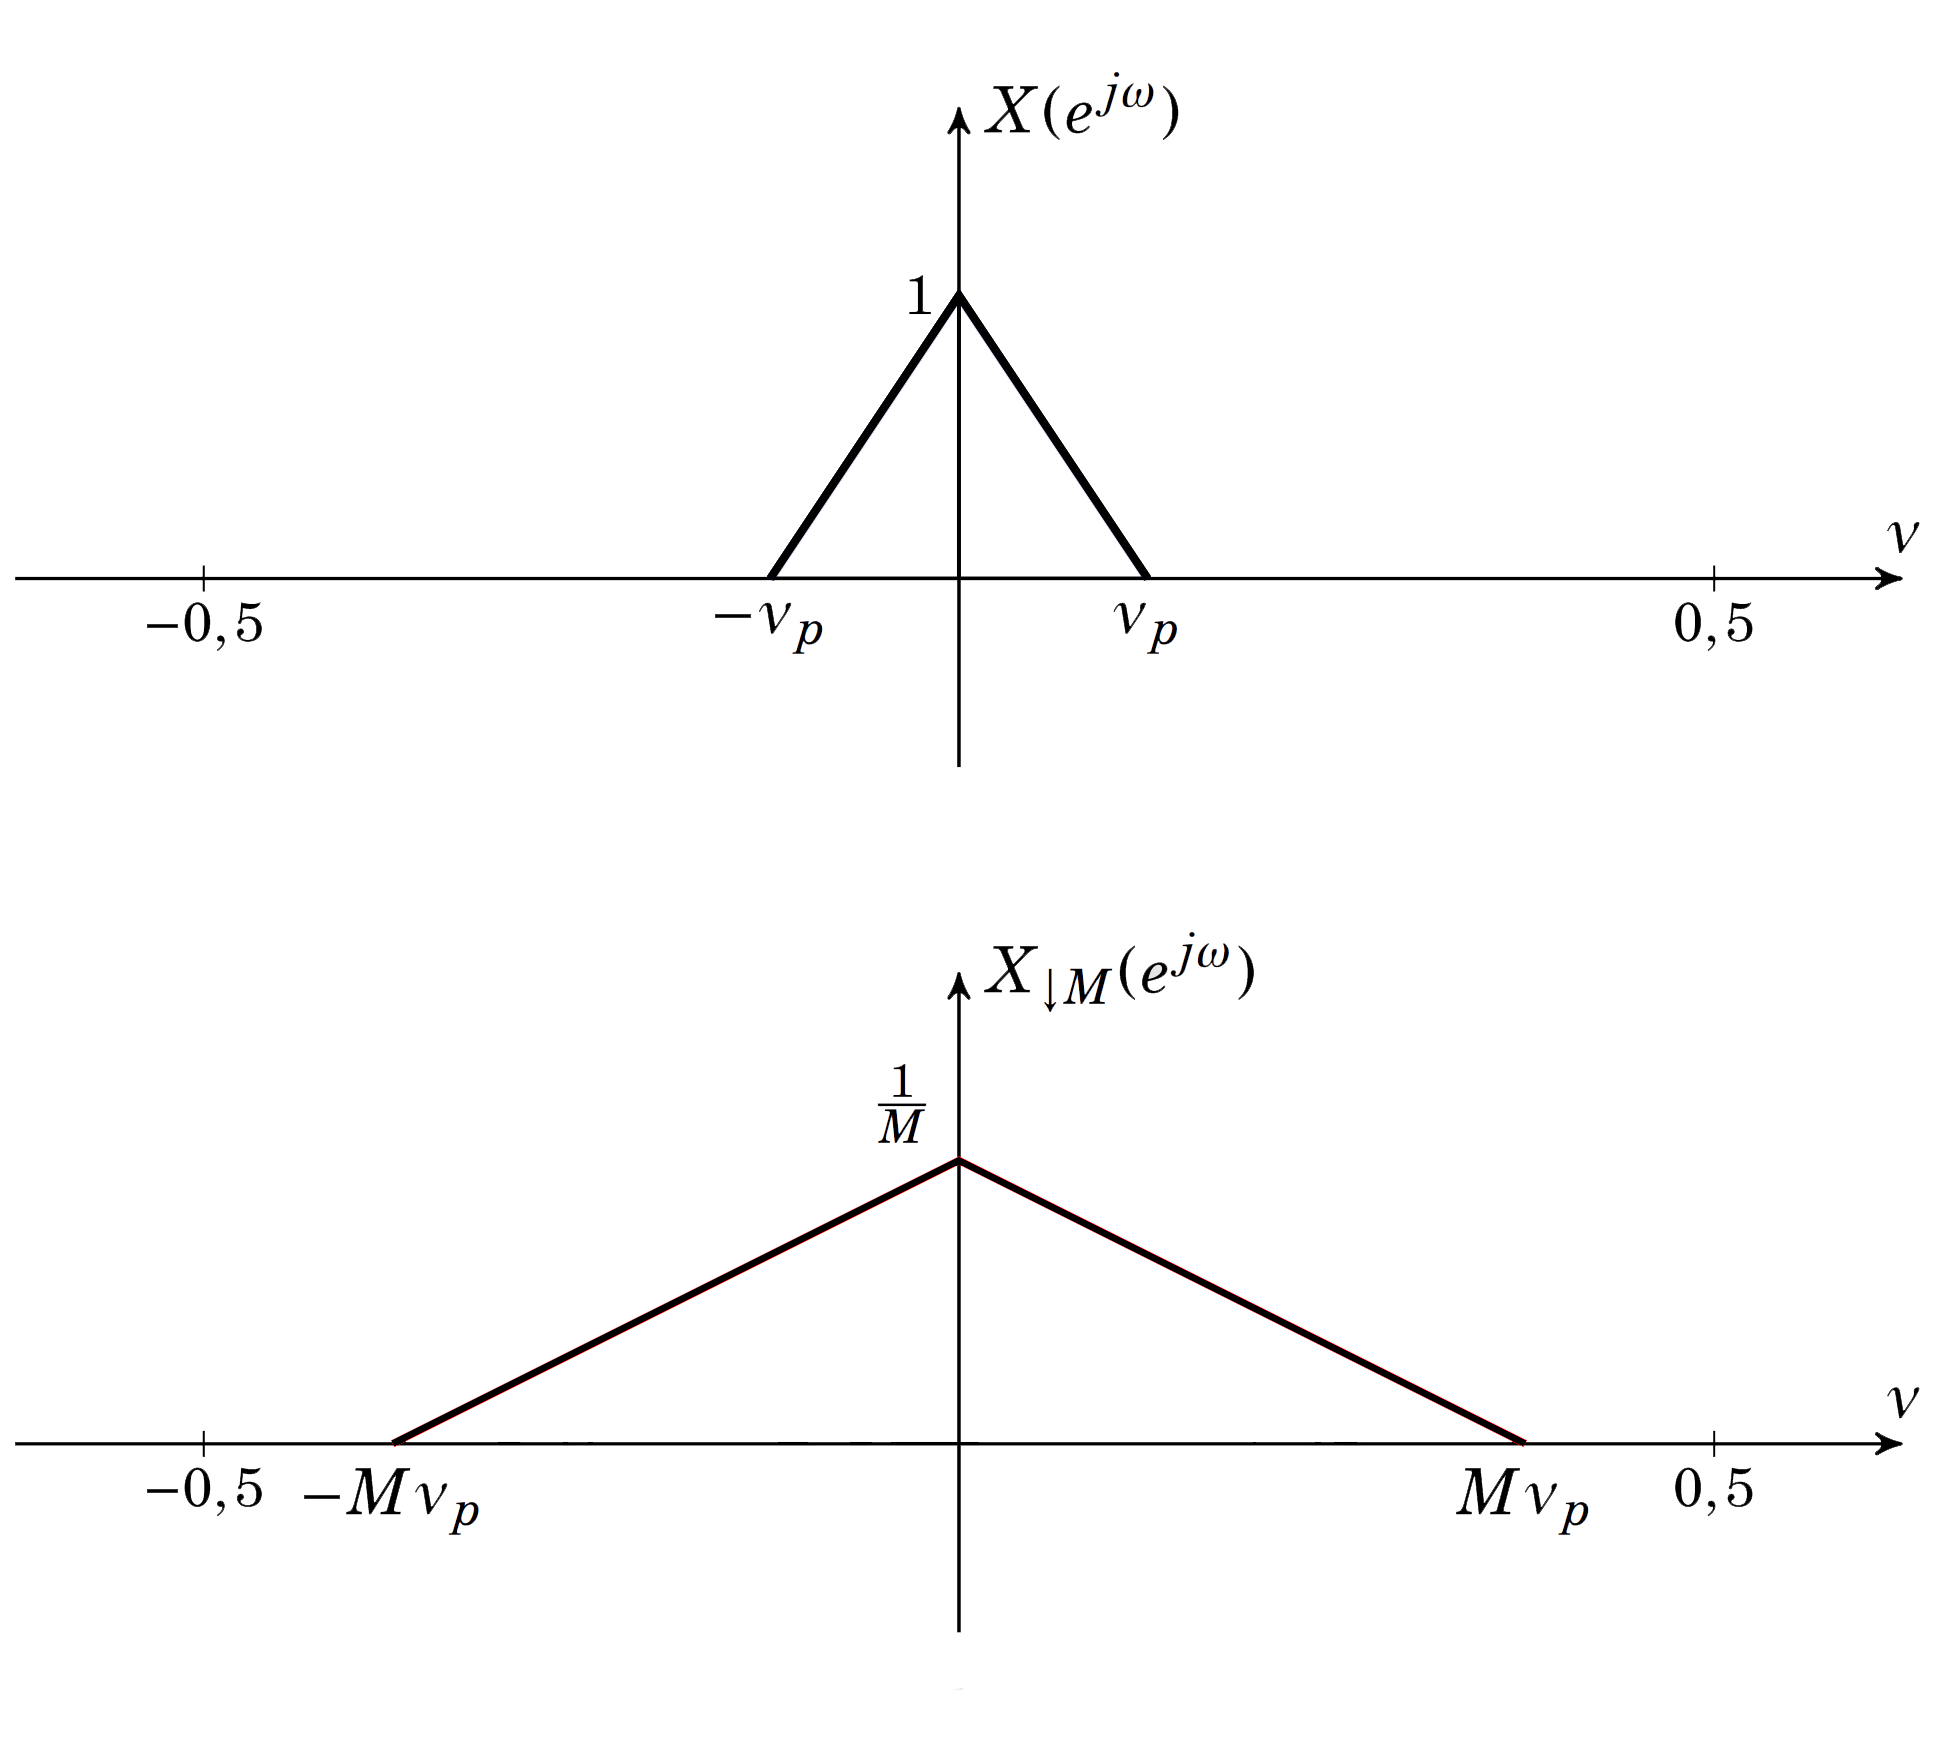
\includegraphics[width=10cm]{Images/Chuong2/pho_truoc_sau_down.png}
    \caption[Phổ tín hiệu trước và sau khi hạ tốc M lần]{\bfseries \fontsize{12pt}{0pt}\selectfont Phổ tín hiệu trước và sau khi hạ tốc M lần}
    \label{pho_truoc_sau_down}
\end{figure}

Trong các trường hợp M lớn sao cho $Mv_p > 0.5$ thì thì vận tốc lấy mẫu này thấp hơn vận tốc lấy mẫu cần thiết theo định lý Nyquist và như thế sẽ xuất hiện hiện tượng chồng phổ. Để giải quyết vấn đề này thì ngay trong miền tín hiệu số, có thể cho tín hiệu gốc $x(n)$ đi qua một bộ lọc thông thấp để dải thông của đầu ra phải nhỏ hơn $0.5/M$. Bộ lọc thông thấp mô tả như hình \ref{filter_downsample} - Hệ thống này có tên là bộ lọc giảm mẫu số (Decimation Filter).

\begin{figure}[ht!]
    \centering
    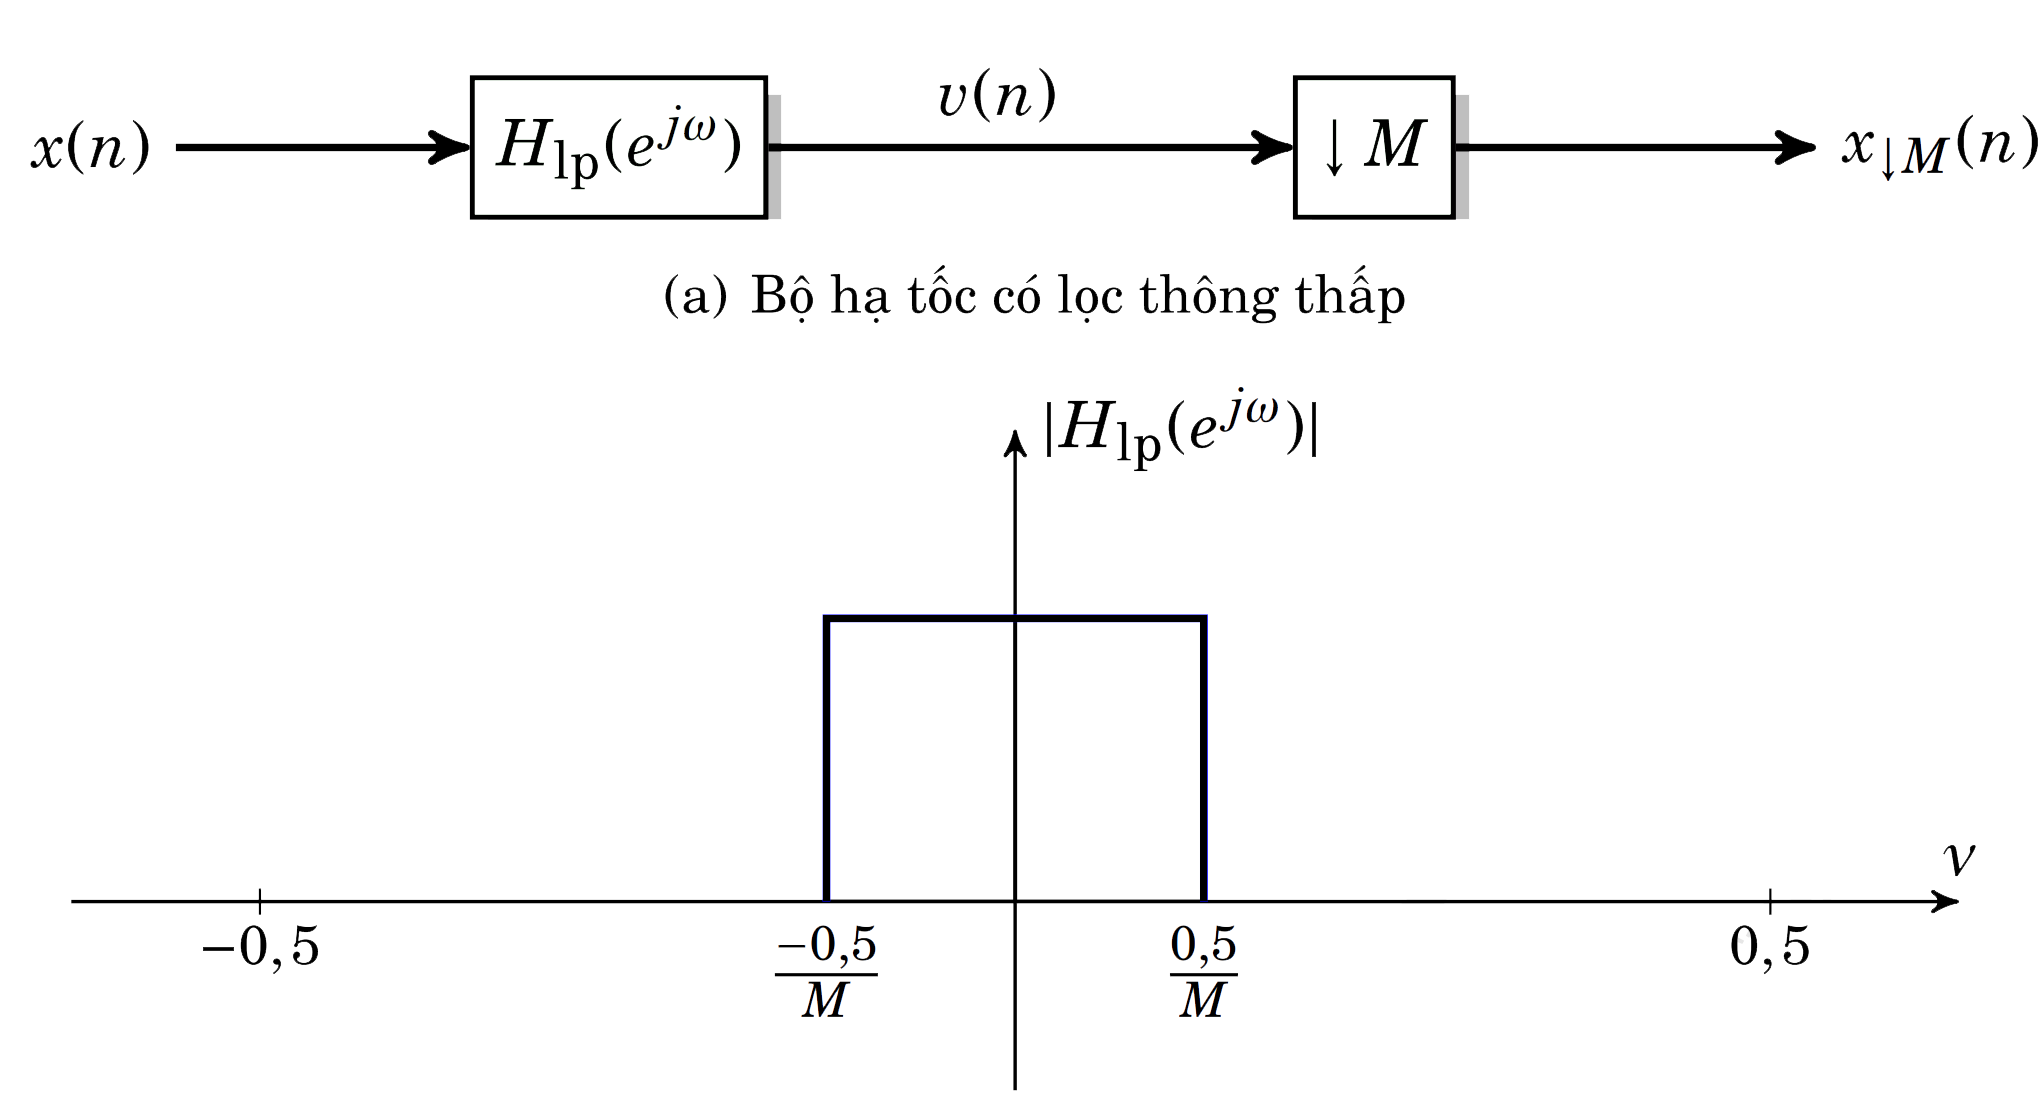
\includegraphics[width=12cm]{Images/Chuong2/filter_downsample.png}
    \caption[Bộ lọc thông thấp để tránh chồng phổ]{\bfseries \fontsize{12pt}{0pt}\selectfont Bộ lọc thông thấp để tránh chồng phổ}
    \label{filter_downsample}
\end{figure}

Nếu tín hiệu số gốc $x(n)$ có dải thông nhỏ hơn tần số cắt $0,5/M$ thì bộ lọc không tác động đến tín hiệu. Tuy nhiên, nếu $x(n)$ có dải thông lớn hơn tần số cắt thì bộ lọc loại phần phổ nằm ngoài tần số cắt. Từ hình trên cho thấy, lúc hạ tốc ta chấp nhận mất một ít thông tin và kết quả này là điều hiển nhiên với quá trình hạ tốc.

 Hình \ref{decimation_without_filtering-no_decimation} mô tả phổ của tín hiệu có 3 sóng hình sin ở 100Hz, 1000Hz và 2800Hz và một số nhiễu được thêm vào, được lấy mẫu ở 10kHz. Sóng hình sin ở 100Hz và 1000Hz có biên độ thấp hơn nhiều so với sóng hình sin ở 2800Hz. 

\begin{figure}[H]
    \centering
    \includesvg[width=14cm]{Images/Chuong2/decimation_without_filtering-no_decimation.svg}
    \caption[Phổ của tín hiệu gốc, không sử dụng giảm mẫu]{\bfseries \fontsize{12pt}{0pt}\selectfont Phổ của tín hiệu gốc, không sử dụng giảm mẫu}
    \label{decimation_without_filtering-no_decimation}
\end{figure}
Sau khi sử dụng hạ tốc (decimation) ở 2x và 4x, phổ lần lượt sẽ có dạng như hình \ref{decimation_without_filtering-2x_4x_decimation}.

Các tín hiệu ở vùng 1250Hz đến 5000Hz không mất đi mà chúng di chuyển về lại dải tần số 0 - 1250Hz, sau khi giảm mẫu. Ví dụ, tín hiệu 2800Hz đã về tần số 2200Hz và 300Hz tương ứng với Decimation 2x và 4x. Các nhiễu cũng tăng lên sau mỗi lần giảm mẫu, nhiễu ở tần số cao cũng sẽ chuyển về ở tần số thấp.
\begin{figure}[H]
    \centering
    \includesvg[width=14cm]{Images/Chuong2/decimation_without_filtering-2x_4x_decimation.svg}
    \caption[Phổ của tín hiệu sau khi Decimation 2x và 4x]{\bfseries \fontsize{12pt}{0pt}\selectfont Phổ của tín hiệu sau khi Decimation 2x và 4x}
    \label{decimation_without_filtering-2x_4x_decimation}
\end{figure}
 
\subsection{Các bộ lọc tiết kiệm tài nguyên sử dụng trong xử lí số tín hiệu trên nhiều miền tần số}
Mục \ref{xulynhieumientanso} đã đề cập rằng, trong xử lí số tín hiệu trên nhiều miền tần số ta cần sử dụng các bộ lọc để loại bỏ các thành phần tần số sẽ bị chồng phổ khi tiến hành Down-Sampling. Và khi áp dụng lên thiết kế số, bắt buộc chúng ta phải lựa chọn các bộ lọc tối ưu để tiết kiệm tài nguyên nhiều nhất có thế. Mục này sẽ giới thiệu các bộ lọc được sử dụng trong đề tài.
\subsubsection{Giới thiệu về bộ lọc thông thấp}
Như đã trình bày ở phần \ref{downsample}, để tránh bị chồng phổ khi Down-Sampling thì lúc đưa tín hiệu vào, thì tín hiệu đó sẽ được xử lý qua một bộ lọc thông thấp.

Bộ lọc thông thấp là một loại bộ lọc tín hiệu được sử dụng để giảm độ phức tạp của tín hiệu, lọc bớt các tần số cao và chỉ giữ lại các tần số thấp hơn một ngưỡng nào đó.

Bộ lọc thông thấp có thể được thiết kế để loại bỏ các tín hiệu có tần số cao hơn một giá trị cụ thể hoặc để giảm bớt tần số cao một cách đồng đều trên toàn bộ tín hiệu. Các loại bộ lọc thông thấp phổ biến bao gồm bộ lọc Butterworth, bộ lọc Chebyshev, bộ lọc Elliptic và bộ lọc FIR (Finite Impulse Response). Các bộ lọc này có thể được áp dụng bằng các thuật toán số để xử lý tín hiệu số hoặc bằng các mạch điện tử để xử lý tín hiệu tương tự.

Hình \ref{thongthap_rf} mô tả đáp ứng tần số của 1 bộ lọc thông thấp, trong đó: độ gợn sóng là giới hạn giữa hai trị số $1 - \delta_p$ và $1 + \delta_p$, tấn số cắt $\omega_p$, độ gợn sóng trong giải triệt có giá trị cực đại $\delta_s$, $[\omega_p, \omega_s]$ là dải chuyển tiếp.
\begin{figure}[H]
    \centering
    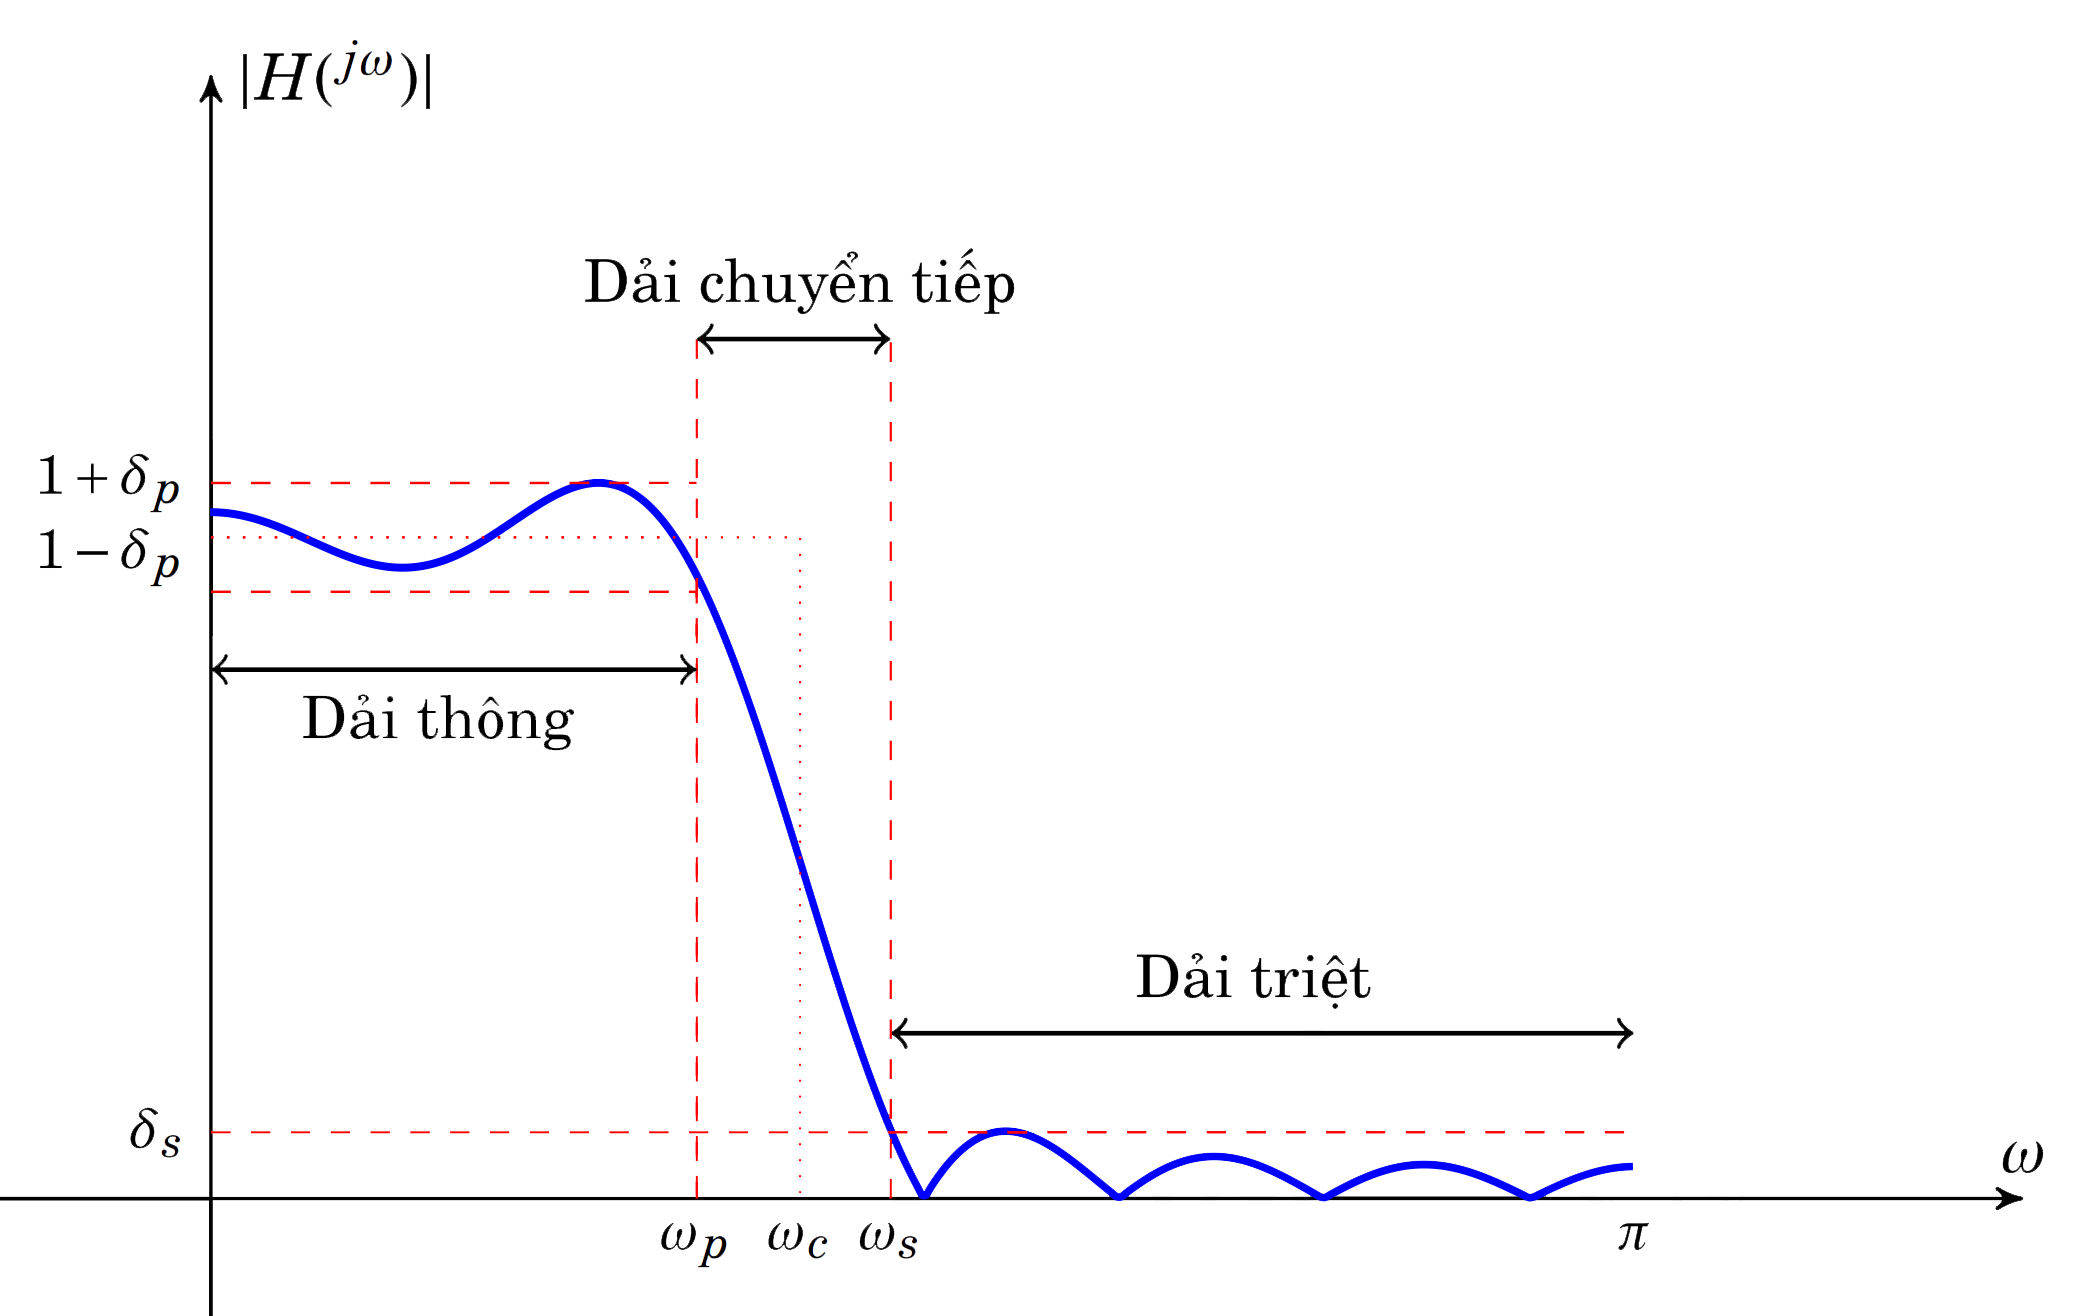
\includegraphics[width=10cm]{Images/Chuong2/thongthap_rf.png}
    \caption[Đáp ứng tần số của một bộ lọc thông thấp]{\bfseries \fontsize{12pt}{0pt}\selectfont Đáp ứng tần số của một bộ lọc thông thấp}
    \label{thongthap_rf}
\end{figure}

\subsubsection{Bộ lọc áp ứng xung hữu hạn -  Finite impulse response (FIR) filter}
Bộ lọc FIR (Finite Impulse Response) là một loại bộ lọc tín hiệu số được sử dụng trong xử lý tín hiệu kỹ thuật số. Bộ lọc FIR có phản hồi xung hữu hạn, nghĩa là phản hồi xung của nó (hoặc phản ứng với bất kỳ đầu vào có độ dài hữu hạn nào) có độ dài hữu hạn, bởi vì nó giảm về 0 trong thời gian hữu hạn. Bộ lọc FIR có thể được sử dụng để thực hiện các tác vụ xử lý tín hiệu như lọc thông qua, lọc chặn, hay trích xuất đặc trưng tín hiệu. Bộ lọc FIR có thể được thiết kế để đáp ứng các yêu cầu xử lý tín hiệu như băng thông, độ lọc và độ trễ. Bộ lọc FIR có thể là rời rạc thời gian hoặc liên tục thời gian và là kỹ thuật số hoặc tương tự. \cite{8256573}
\begin{figure}[H]
    \centering
    \includesvg[width=9cm]{Images/Chuong2/FIR_Filter.svg}
    \caption[Cấu trúc của bộ lọc FIR]{\bfseries \fontsize{12pt}{0pt}\selectfont Cấu trúc của bộ lọc FIR}
    \label{FIR_Filter}
\end{figure}
Một bộ lọc FIR rời rạc thời gian tính đầu ra bằng cách tính tổng trọng số của một số lượng đầu vào đã cho gần đây nhất (phương trình \ref{fir}).
\begin{equation}\label{fir}
       y[n]= b_0x[n] + b_1x[n-1] + b_2x[n-2] + ... + b_Nx[n-N] = \sum^{N}_{i=0}b_ix[n - i]
\end{equation}
Trong đó:
\begin{itemize}
  \item $x[n]$ là tín hiệu đầu vào.
  \item $y[n]$ là tín hiệu đầu ra.
  \item $N$ là số tầng của bộ lọc).
  \item $b_i$ là giá trị của đáp ứng xung thời điểm thứ $i$ với $0 \leq i \leq N$, cũng được gọi là hệ số của bộ lọc.
\end{itemize}

Các $x[n-i]$ trong thuật ngữ còn gọi là "taps". 

Đáp ứng xung của bộ lọc được xác định là khác 0 trong một khoảng thời gian hữu hạn. Bao gồm các số 0, đáp ứng xung là chuỗi vô hạn (phương trình \ref{duxfir}).
\begin{equation}\label{duxfir}
    h[n] = \sum ^{N}_{i=0}b_i\delta[n-i]=\left\{\begin{matrix}b_n,& 0 \leq n \leq N
    \\&
\\ 0, & \text{khác}
\end{matrix}\right.
\end{equation}

Các ưu điểm của bộ lọc FIR có thể kể đến bao gồm:
\begin{itemize}
\item Tính ổn định: Bộ lọc FIR là ổn định vì nó không có phản hồi nội tại, điều này đảm bảo rằng đầu ra không bị dao động hoặc không hội tụ.
\item Tính ngắt mạnh: Bộ lọc FIR có tính chất ngắt mạnh, có thể đạt được bằng cách đặt các trọng số của bộ lọc bằng 0.
\item Dễ dàng thiết kế: Bộ lọc FIR có thể được thiết kế dễ dàng vì nó không có phản hồi nội tại và chỉ yêu cầu thực hiện các phép tính toán đơn giản như cộng và nhân.
\item Khả năng đáp ứng yêu cầu chính xác về tần số: Bộ lọc FIR có thể được thiết kế để đáp ứng các yêu cầu chính xác về tần số, nhờ vào tính chất phản hồi xung hữu hạn của nó. Tuy nhiên, độ chính xác này phụ thuộc vào số lượng và bậc của bộ lọc.
\item Có thể được thực hiện bằng cách sử dụng cấu trúc song song: Bộ lọc FIR có thể được thực hiện bằng cách sử dụng cấu trúc song song, điều này có nghĩa là các phép tính có thể được thực hiện song song trên nhiều mẫu đầu vào cùng một lúc, giúp tăng tốc độ xử lý.
\end{itemize}

Bộ lọc FIR được thiết kế bằng cách tìm các hệ số và thứ tự bộ lọc đáp ứng các thông số kỹ thuật nhất định, có thể trong miền thời gian hoặc miền tần số (phổ biến nhất). Các bộ lọc phù hợp thực hiện mối tương quan chéo giữa tín hiệu đầu vào và dạng xung đã biết. Tích chập FIR là mối tương quan chéo giữa tín hiệu đầu vào và bản sao đảo ngược thời gian của đáp ứng xung. Do đó, đáp ứng xung của bộ lọc phù hợp được "thiết kế" bằng cách lấy mẫu dạng xung đã biết và sử dụng các mẫu đó theo thứ tự ngược lại làm hệ số của bộ lọc. \cite{signalsystem}

Các phương pháp thiết kế phố biến hiện nay như phương pháp thiết kế cửa số, lấy mẫu tần số, Parks–McClellan,  bằng thuật toán DFT, 	\ldots Do phạm vi đề tài nên các phương pháp này sẽ được trình bày và nói rõ chi tiết ở \cite{TAN2014xiii}.

\subsubsection{Bộ lọc CIC -  Cascaded Integrator Comb} \label{cic_filter_ref}
Khi nghiên cứu chủ đề chuyển đổi PDM sang PCM, chúng ta không thể bỏ qua về bộ lọc lược tích hợp xếp tầng (CIC), bởi vì chúng cực kỳ nhẹ về mặt tài nguyên, nhờ một số thủ thuật và chuyển đổi. Mục này sẽ trình bày cái nhìn tổng quan về bộ lọc trung bình động và cách tối ưu bộ lọc trung bình động sang bộ lọc CIC.
\paragraph{Bộ lọc trung bình động - Moving Average Filters}\label{maf}
Các bộ lọc FIR điển hình có độ dài nhất định hoặc các "taps" và mỗi tap yêu cầu một phép nhân và một phép cộng. Các hệ số nhân ở đó để định hình bộ lọc sao cho nó có các đặc tính dải thông, dải chuyển tiếp và dải triệt mong muốn. Việc áp dụng FIR nhiều tap lên phần cứng có thể tiêu tốn rất nhiều tài nguyên và điều đó không hiệu quả. Vì vậy chúng ta cần triển khai các bộ lọc loại bỏ các phép toán phức tạp. Khi đó lựa chọn đơn giản nhất là bộ lọc trung bình động - Moving Average Filters. Bộ lọc thực hiện cực kỳ đơn giản, nó tính tổng của N mẫu đến cùng và chia nó cho N.
\begin{figure}[H]
    \centering
    \includesvg[width=13cm]{Images/Chuong2/moving_average_filter_overview_linear.svg}
    \caption[Đáp ứng tần số của bộ lọc trung bình động ở các cấu hình khác nhau - theo đơn vị tuyến tính]{\bfseries \fontsize{12pt}{0pt}\selectfont Đáp ứng tần số của bộ lọc trung bình động ở các cấu hình khác nhau - theo đơn vị tuyến tính}
    \label{moving_average_filter_overview_linear}
\end{figure}
Bộ lọc trung bình động có lẽ là một trong những bộ lọc phổ biến nhất trong xử lý tín hiệu số. Nó không hề khó để hiểu và triển khai, chúng đối xứng nên có đáp ứng pha tuyến tính và đây cũng là bộ lọc tối ưu để giảm nhiễu trắng. (Đó là bởi vì nhiễu trắng không tác động đến mẫu này hay mẫu khác, nó ảnh hưởng đến bất kỳ mẫu nào với cơ hội như nhau. Và do đó, không có cách nào bạn có thể điều chỉnh hệ số này hoặc hệ số kia của các hệ số bộ lọc theo một số cách ưu tiên.)

Các bộ lọc trung bình động cũng có một số nhược điểm lớn: chúng có độ suy giảm lớn trong dải thông, chúng có tốc độ chuyển từ dải thông sang dải dừng rất chậm, chúng có hành vi trong miền thời gian không tốt (đổ chuông) và sự suy giảm băng tần dừng cũng rất thấp. Tuy nhiên, chúng ta có thể khắc phục sự suy giảm dải triệt thấp bằng cách xếp tầng nhiều bộ lọc nối tiếp nhau, mặc dù điều đó cũng làm cho sự suy giảm dải thông trở nên tồi tệ hơn.

Vì các hệ số bộ lọc là cố định và không đổi nên chỉ có 2 tham số để xử lý: kích thước của hộp lấy mẫu và thứ tự và số lượng bộ lọc được xếp tầng.
\begin{figure}[H]
    \centering
    \includesvg[width=13cm]{Images/Chuong2/moving_average_filter_overview.svg}
    \caption[Đáp ứng tần số của bộ lọc trung bình động ở các cấu hình khác nhau - theo đơn vị dB]{\bfseries \fontsize{12pt}{0pt}\selectfont Đáp ứng tần số của bộ lọc trung bình động ở các cấu hình khác nhau - theo đơn vị dB}
    \label{moving_average_filter_overview}
\end{figure}
Vì đáp ứng xung của bộ lọc là hình hộp chữ nhật nên đáp ứng tần số của nó sẽ biểu diễn theo hàm $sinc(f)$ như hình \ref{moving_average_filter_overview_linear} với tần số chuẩn hóa từ $[0, 1/2 F_s]$. Khi chúng ta tăng chiều dài của bộ lọc, mọi thứ sẽ bị ép sang trái: dải thông trở nên hẹp hơn. Và khi tăng số tầng của các bộ lọc thì độ suy giảm của dải triệt sẽ tăng lên. Có thể thấy rõ hơn đáp ứng tần số theo đơn vị dB ở hình \ref{moving_average_filter_overview}.

\paragraph{Từ bộ lọc trung bình động đến bộ lọc CIC}
Từ kiến trúc bộ lọc trung bình, tác giả Hogenauer đã đưa ra kiến một kiến trúc có tên là CIC (Cascaded Integrator Comb) sử dụng trong xử lí số tín hiệu trên nhiều miền tần số\cite{CIC}.

Bắt đầu với bộ lọc trung bình động với độ dài bằng 4 có kiến trúc được mô tả như hình \ref{cic_1}.
\begin{figure}[H]
    \centering
    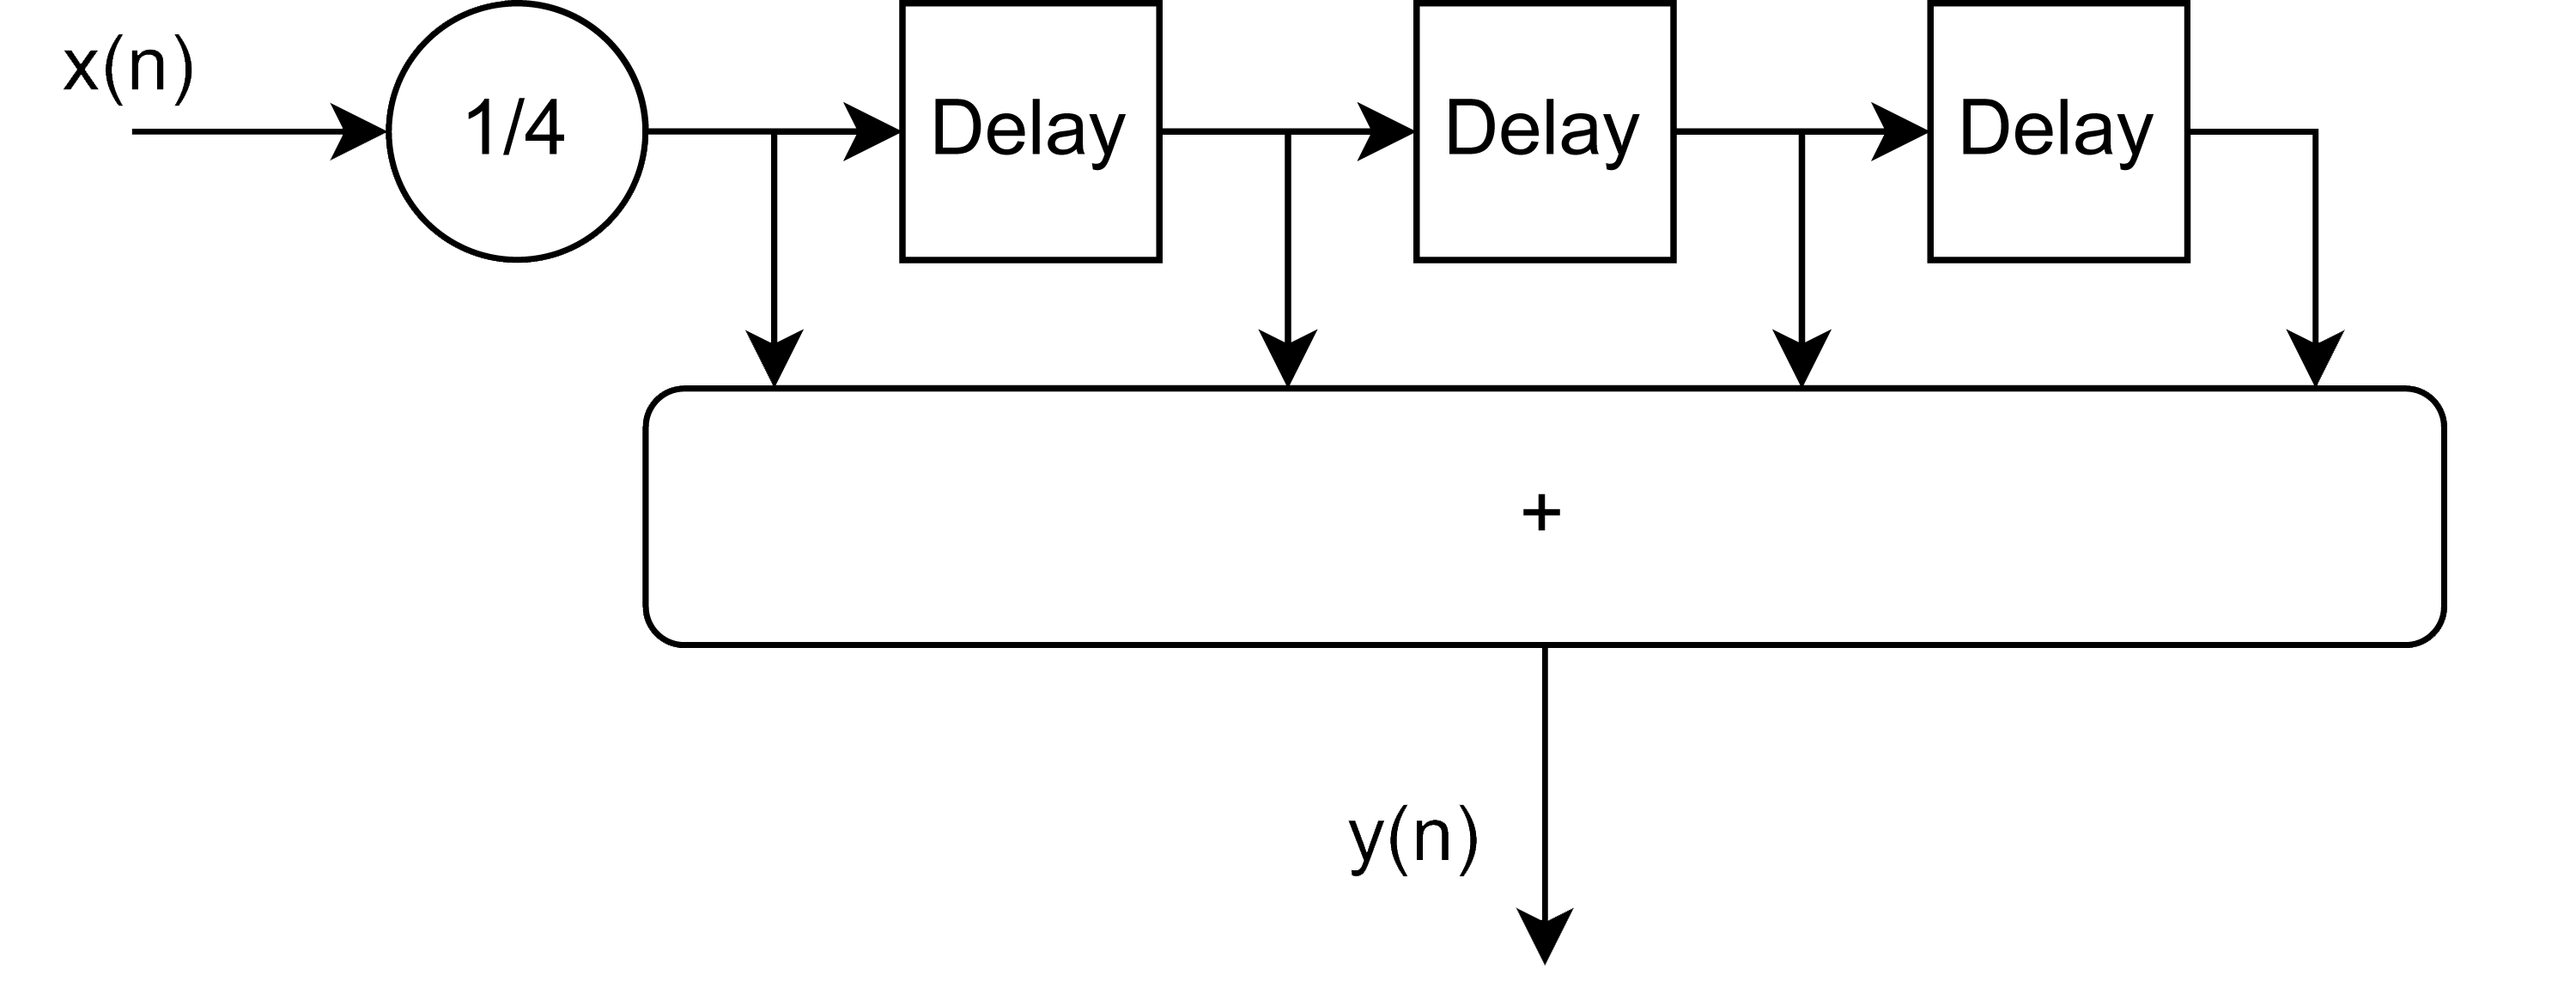
\includegraphics[width=8cm]{Images/Chuong2/cic/cic_1.png}
    \caption[Kiến trúc của bộ lọc trung bình động với chiều dài bằng 4]{\bfseries \fontsize{12pt}{0pt}\selectfont Kiến trúc của bộ lọc trung bình động với chiều dài bằng 4}
    \label{cic_1}
\end{figure}

Việc thực hiện trên trung bình 4 mẫu, yêu cầu 3 phần tử trễ và 3 bộ cộng. Và hành động chia ban đầu cho 4 là để đảm bảo rằng bộ lọc có mức tăng đơn vị. 

Như đã đề cập ở phần trên, không có số nhân trong thiết kế này, nhưng 3 bộ cộng hơi khó có thể được chấp nhận, đặc biệt vì con số đó sẽ tăng lên tương ứng đối với các bộ lọc trung bình động có độ dài dài hơn. Từ \cite{cic_opt}, bộ lọc trung bình động đã được tối ưu và đưa ra kiến trúc CIC như hình \ref{cic_7}.

\begin{figure}[H]
    \centering
    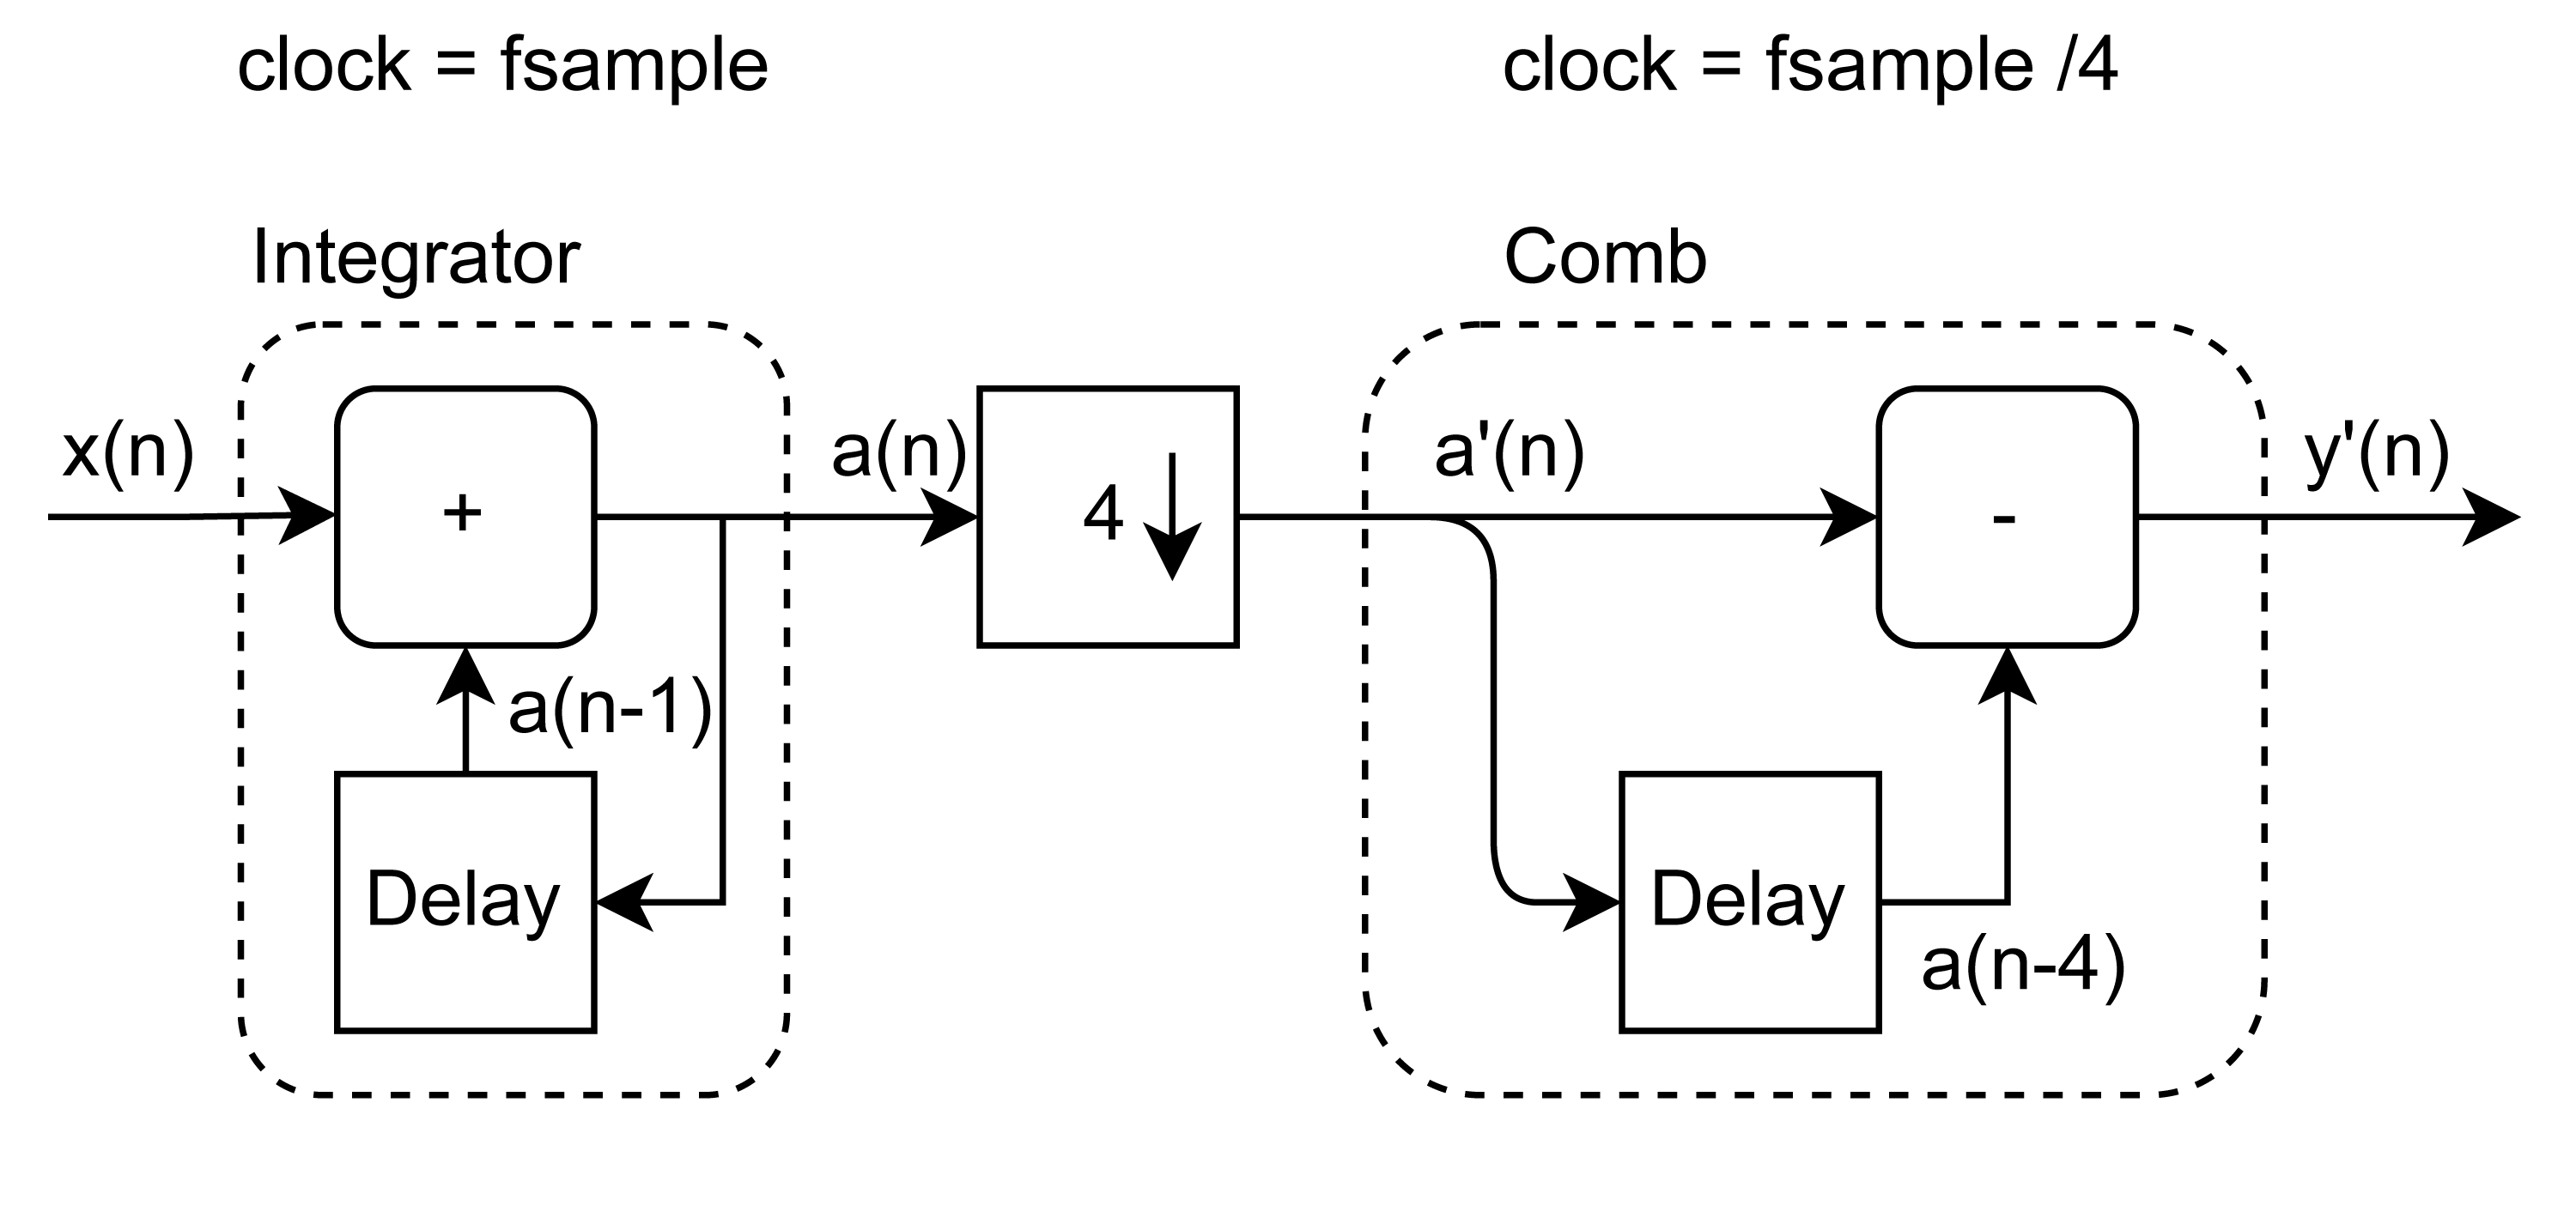
\includegraphics[width=10cm]{Images/Chuong2/cic/cic_7.png}
    \caption[Kiến trúc giản lược của bộ lọc trung bình động với decimation]{\bfseries \fontsize{12pt}{0pt}\selectfont Kiến trúc giản lược của bộ lọc trung bình động với decimation}
    \label{cic_7}
\end{figure}

Khi sử dụng decination (hạ tần), bộ lọc trung bình động có thiết kế ban đầu bao gồm $N$ bộ trễ, $N-1$ bộ cộng chạy ở tần số mẫu đầu vào đã giảm xuống chỉ còn 2 bộ trễ, 1 bộ cộng, 1 bộ trừ và 1 nửa kiến trúc chạy với tốc độ lấy mẫu đầu ra. Thiết kế mới này được gọi là bộ lọc CIC - Cascaded Integrator Com.

Đối với các bộ CIC nhiều tầng, chúng ta chỉ việc cần thêm các khối "comb" và "integrator" và nhóm chúng lại cùng một thứ tự. Hình \ref{cic_8} là ví dụ của một bộ lọc CIC decimation 3 tầng.
\begin{figure}[H]
    \centering
    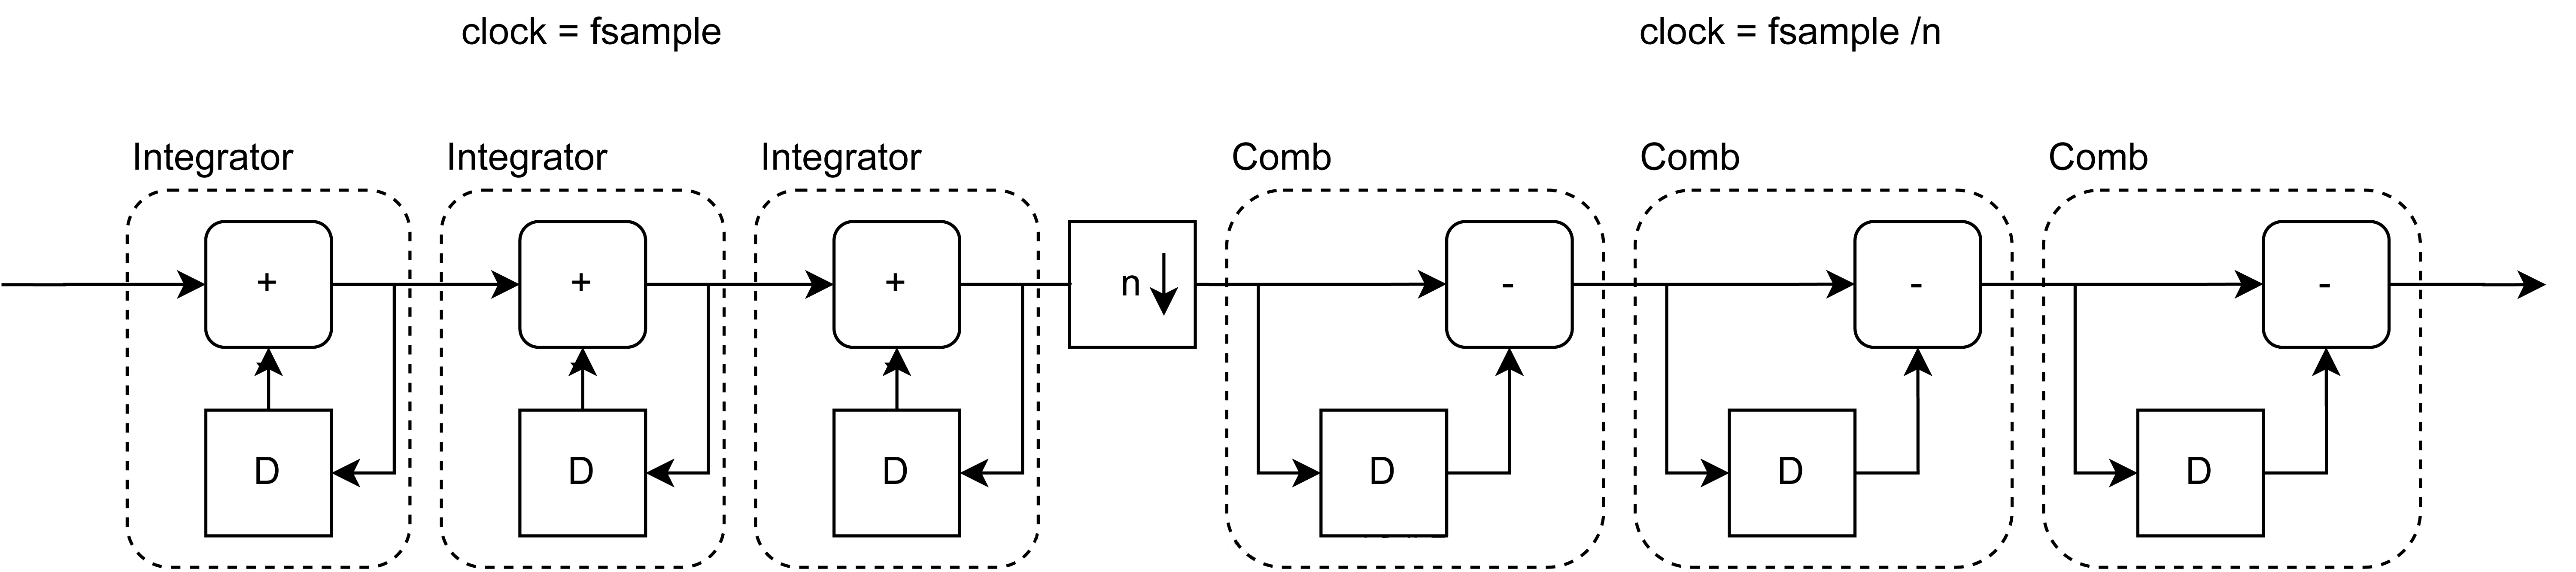
\includegraphics[width=14cm]{Images/Chuong2/cic/cic_8.png}
    \caption[Kiến trúc của bộ lọc CIC 3 tầng ]{\bfseries \fontsize{12pt}{0pt}\selectfont Kiến trúc của bộ lọc CIC 3 tầng}
    \label{cic_8}
\end{figure}
\paragraph{Các đặc điểm của bộ lọc CIC}
Bây giờ chúng ta đã biết tại sao các bộ lọc trung bình động lại rất phổ biến đối với phép hạ tần - decimation, việc triển khai CIC hầu như không yêu cầu tài nguyên, bất kể tỷ lệ lấy mẫu lên hoặc xuống. Điều đó phù hợp cho việc tổng hợp và triển khai trên các nền tảng FPGA.

Tuy nhiên, các nhược điểm của các bộ lọc trung bình động đã được đề cập ở mục \ref{maf}, độ suy giảm dải dừng kém và độ suy giảm dải thông không phẳng không thể biến mất.

Trên thực tế, trong bộ lọc CIC decimation, độ dài của bộ lọc trung bình động phải là bội số nguyên của tỷ lệ hạ tần - decimation ratio. Trong hầu hết các trường hợp, tỷ lệ đó là 1. Do đó, cách duy nhất để tác động đến sự suy giảm của dải triệt là tăng số lượng bộ "comb" và "integrator", tuy nhiên điều đó cũng làm tăng sự suy giảm của dải thông.

\textbf{Kích thước của các phần tử trễ trong bộ lọc CIC}

Nếu các phần tử trễ của bộ lọc CIC không đủ lớn, bộ lọc sẽ bị tràn làm sai đầu ra. Cách dễ nhất để tránh lỗi này là cung cấp cho tất cả bộ trễ cùng một kích thước. Việc tính độ dài bit của các bộ trễ thể hiện như công thức \ref{bitcic}.

\begin{equation} \label{bitcic}
    n_r = I + [M \times log_2(N \times R)] (bits)
\end{equation}

Trong đó:
\begin{itemize}
    \item $I$: chiều dài bit của đầu vào (bits)
    \item $M$: Số tầng của bộ lọc
    \item $N$: số thanh ghi delay trong 1 tầng
    \item $R$: Hệ số decimation
\end{itemize}
\subsubsection{Bộ lọc Half-Band (Half-Band Filters)}
Bộ lọc Half-band là một loại bộ lọc tín hiệu kỹ thuật số trong đó băng thông của tín hiệu đầu vào được chia thành hai phần bằng nhau, và băng thông thấp của tín hiệu được lọc ra trong phạm vi từ 0 đến một nửa của tần số lấy mẫu, trong khi băng thông cao của tín hiệu được bỏ qua.

Một cách đơn giản, một half-band filter là bộ lọc được thiết kế để giảm đáng kể số lượng thông tin được truyền trong tín hiệu đầu vào. Bộ lọc này có thể được sử dụng để giảm độ phân giải của tín hiệu và giảm chi phí tính toán khi xử lý tín hiệu.

 Hiệu quả của bộ lọc half-band phát sinh từ việc khoảng 50\% hệ số bộ lọc là bằng không (giảm được 50\% phép nhân), do đó, giảm chi phí triển khai. \cite{half_band}

 Khi chúng ta bắt đầu với tốc độ lấy mẫu $F_s$, băng thông của tín hiệu đó sẽ đi từ $0$ đến $F_s/2$. Bộ lọc Half-band được sử dụng để giảm băng thông xuống $F_s/4$. Điều thú vị ở đây là đáp ứng tần số của bộ lọc đối xứng cả theo trục tần số và trục cường độ, hình \ref{half_band_symmetry}.
\begin{figure}[ht!]
    \centering
    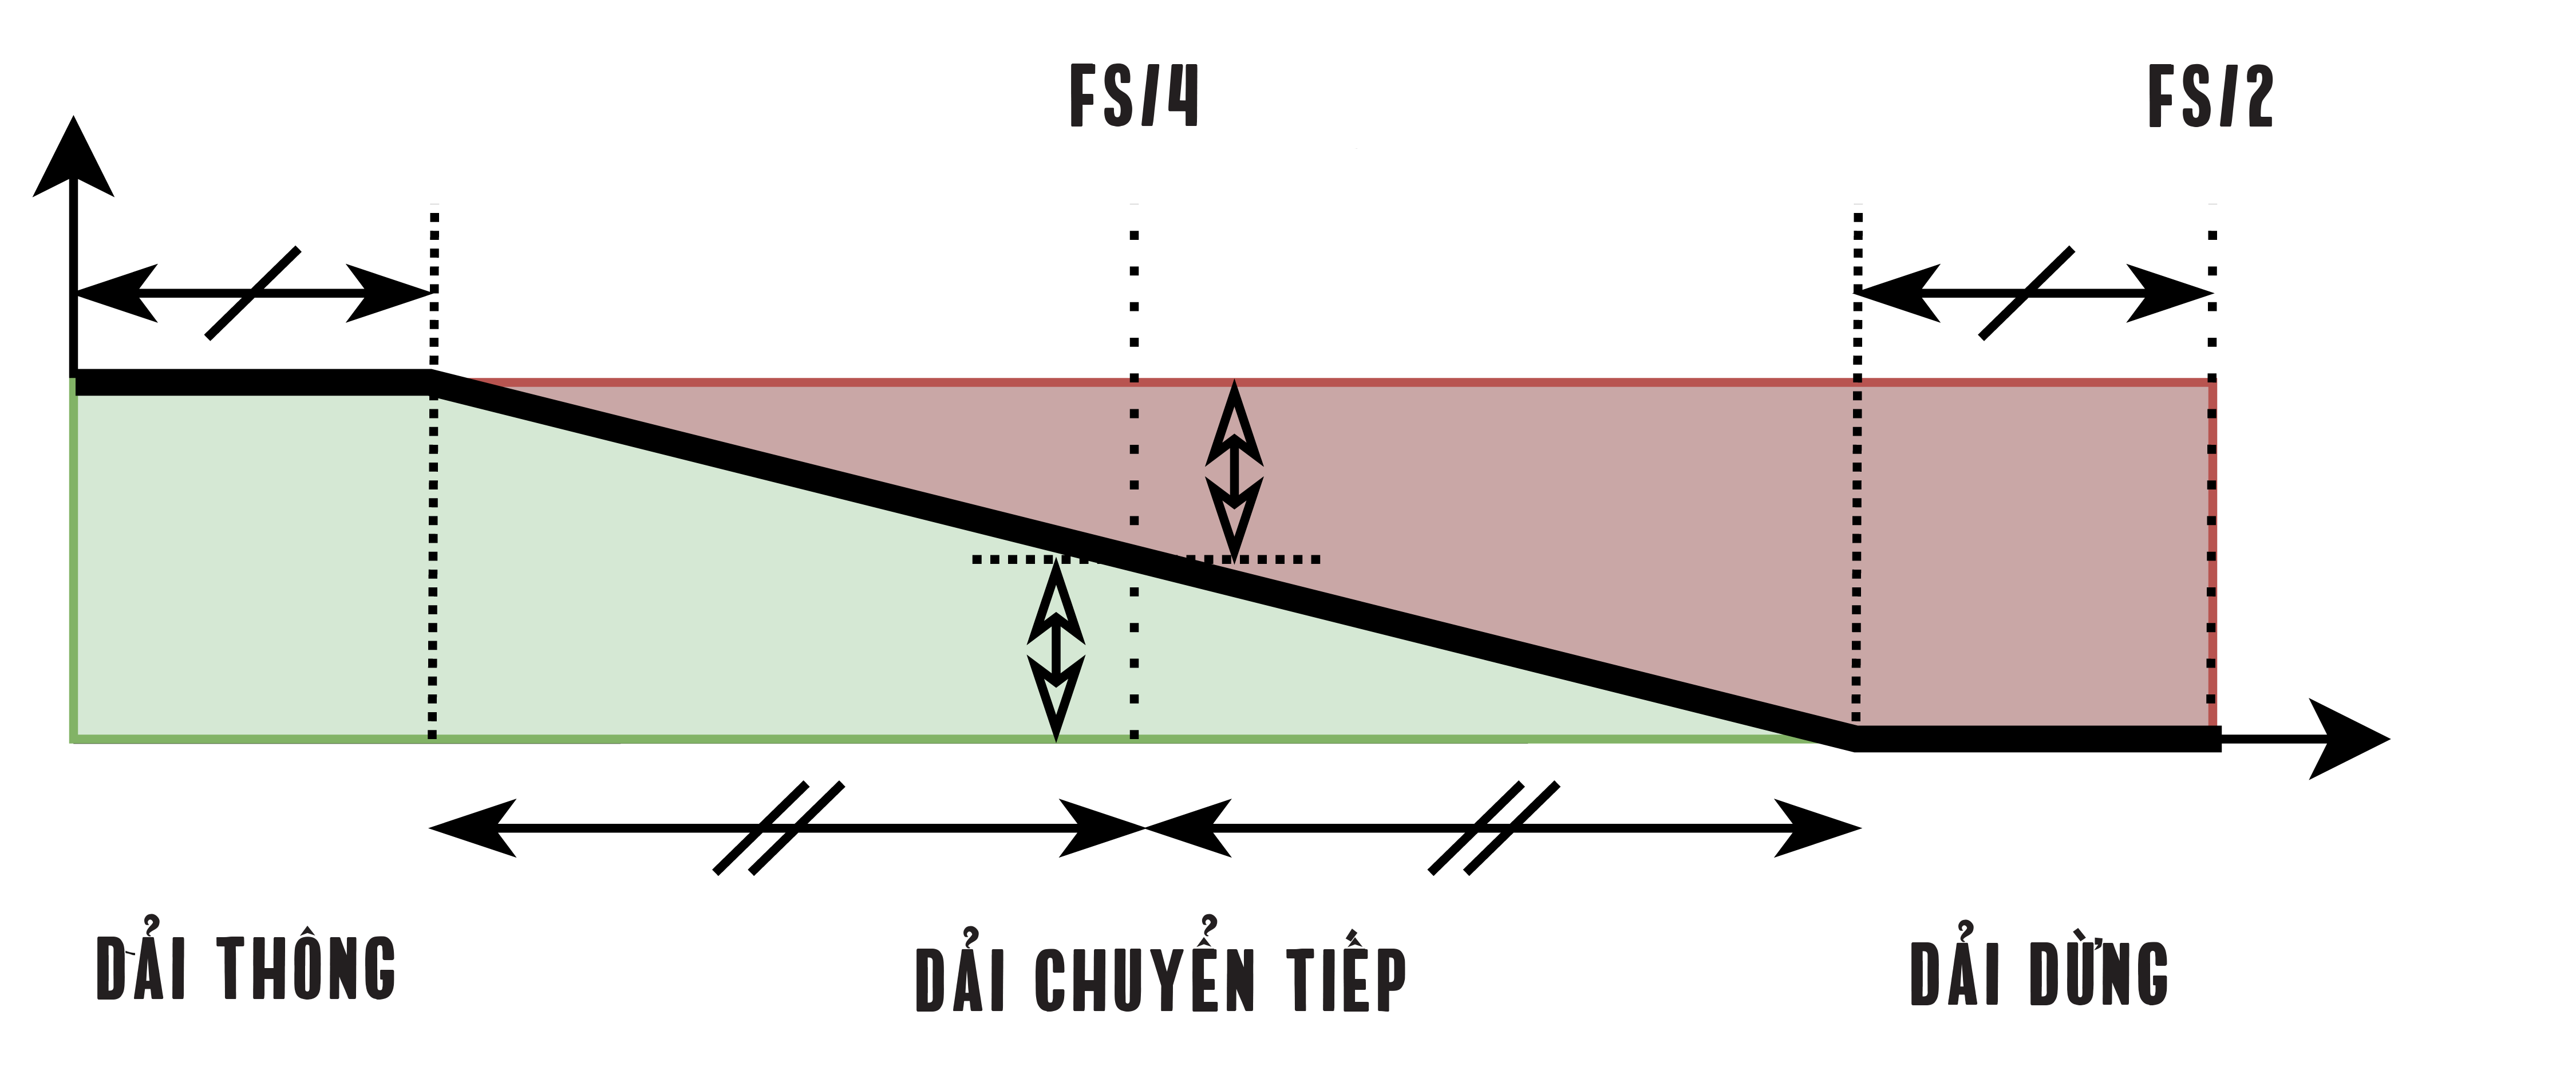
\includegraphics[width=12cm]{Images/Chuong2/halfband-half_band_symmetry.png}
    \caption[Đáp ứng tần số của bộ lọc Half-band]{\bfseries \fontsize{12pt}{0pt}\selectfont Đáp ứng tần số của bộ lọc Half-band}
    \label{half_band_symmetry}
\end{figure}

Với $H(z)$ là hàm truyền đạt của một bộ lọc Half-band có $N-1$ tầng. $H(z)$ được biểu diễn như công thức \ref{hb_ct1}.

\begin{equation}\label{hb_ct1}
    H(z) = \sum^{N-1}_{n = 0}h(n)x^{n-1}
\end{equation}

Với đáp ứng tần số $H(e^{-j\omega})$ được biểu diễn bằng công thức \ref{hb_ct2}. Với $H_0(e^{j\omega})$ là đáp ứng biên độ, biểu diễn như hình \ref{hb_1}. Để thể hiện đối xứng thì tần số cắt $\pi/2$, $\omega_p + \omega_s = \pi$ và độ gợn sóng $\delta_1=\delta_2=\delta$.

\begin{equation}\label{hb_ct2}
    H(e^{j\omega}) = H(e^{-j\omega N - 1/2})H_0(e^{j\omega}) 
\end{equation}

\begin{figure}[ht!]
    \centering
    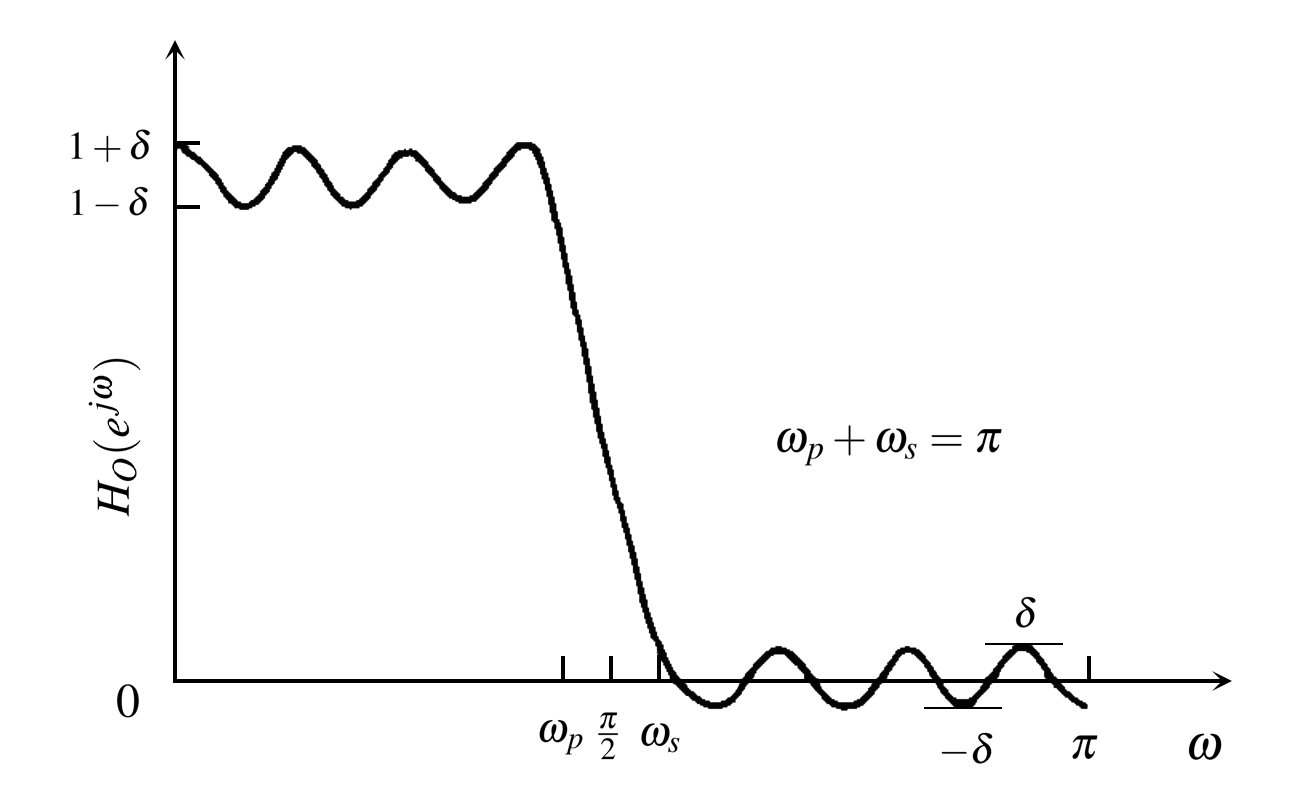
\includegraphics[width=10cm]{Images/Chuong2/half-band.png}
    \caption[Đáp ứng biên độ cơ bản của bộ lọc Half-band]{\bfseries \fontsize{12pt}{0pt}\selectfont Đáp ứng biên độ cơ bản của bộ lọc Half-band}
    \label{hb_1}
\end{figure}

Lúc này đáp ứng xung của bộ lọc Half-band sẽ tính bằng công thức \ref{hb_ct3}.
\begin{equation}\label{hb_ct3}
 h(n)=\left\{\begin{matrix}
0, & \displaystyle n - \frac{N-1}{2} = & \text{lẻ và khác không}\\ 
& &\\ 
\displaystyle \frac{1}{2},& n = \displaystyle \frac{N-1}{2} &
\end{matrix}\right.
\end{equation}

Cách đơn giản nhất để thiết kế các bộ lọc Half-band là sử dụng thuật toán McClellan-Parks \cite{rao2018digital} được sử dụng rộng rãi với các thông số thỏa mãn $\omega_p + \omega_s = \pi$ và độ gợn sóng $\delta_1=\delta_2=\delta$. Một số thủ thuật thiết kế sẽ được trình bày chi tiết ở \cite{half_band}.

\begin{figure}[ht!]
    \centering
    \includesvg[width=12cm]{Images/Chuong2/half_band_example.svg}
    \caption[Đáp ứng tần số cường độ và đáp ứng xung của bộ lọc Half-band]{\bfseries \fontsize{12pt}{0pt}\selectfontĐáp ứng tần số và đáp ứng xung của bộ lọc Half-band}
    \label{half_band_example}
\end{figure}
Hình \ref{half_band_example} là một ví dụ của bộ lọc Half-band ngẫu nhiên. Ta có thể thấy, biểu đồ đối xứng quanh điểm có tọa độ $(0.25, 0.5)$, độ gợn sóng của dải thông và dải dừng đều là $0.1$, các hệ số ở vị trí lẻ đều bằng 0 và hệ số của tap trung tâm bằng $1/2$.

\subsection{Tính toán Fixed-point}
Trong phần mềm, các phép tính toán truyền thống với số dấu phẩy động đều thực hiên trên GPU hay CPU, ví dụ sử dụng kiểu float-32. Khi triển khai ở cấp độ phần cứng các tính toán dấu phẩy động sẽ chậm hơn so dấu phẩy tĩnh do đó rất khó kiểm soát phần định trị và số mũ cho các phép toán khác nhau.
\begin{equation} \label{fbct}
    x_b = x \times 2^N
\end{equation}

Biểu diễn fixed-point như công thức \ref{fbct}, trong đó: $x$ là số thực. Tiến hành nhân $2^N$ để chuẩn hóa $x_b$ thành số nguyên. Điều đó đồng nghĩa chúng ta phải chia cho $2^N$ để được giá trị thực hoặc chỉ cần dịch đi $N$ vị trí.
\subsection{Kết luận chương}
Qua \hyperref[chuong2]{chương 2}, chúng ta đã có đủ các thành phần cần thiết để tiến hành thiết kế bộ chuyển đổi PDM sang PCM bằng thiết kế số. Trong chương tiếp theo, chúng ta sẽ tập hợp các lý thuyết đã trình bày ở trên và triển khai một cách cụ thể.
\newpage